% !TEX program = xelatex
% ============================================================================
% មគ្គុទ្ទេសក៍គរុកោសល្យគ្រូ និងសេណារីយ៉ូបង្រៀនលម្អិត (Teacher's Guideline — HL & Incenter)
% មុខវិជ្ជា៖ គណិតវិទ្យា ថ្នាក់ទី៨ — មេរៀនទី១២៖ ការប្រៀបធៀបត្រីកោណ
% ចំណុចរង៖ ១.៣.២ ករណីត្រីកោណកែង អ.ជ (HL) និងប្រសព្វពុះមុំក្នុងត្រីកោណ (ទំ.១៥៤--១៥៦, ១៦៥)
% គ្រូបង្រៀន៖ ហុក ប៊ុនថែន | អនុវិទ្យាល័យព្រះក្រសាំង (កំពង់ស្វាយ-កំពង់ធំ)
% ============================================================================
\documentclass[a4paper,12pt]{article}

\usepackage[a4paper, left=1.55cm, right=1.55cm, top=2.30cm, bottom=2.30cm, headheight=20pt, headsep=0.68cm, footskip=0.88cm]{geometry}
\usepackage{amsmath, amssymb}
\usepackage{unicode-math}
\usepackage{fontspec}
\usepackage{array, longtable, multirow, colortbl, booktabs}
\usepackage[table]{xcolor}
\usepackage{enumitem}
\usepackage{pifont}
\usepackage{fancyhdr}
\usepackage{lastpage}
\usepackage{needspace}
\usepackage[hyphens]{url}
\usepackage{tikz}
\usepackage[most]{tcolorbox}
\usetikzlibrary{calc, arrows.meta, angles, quotes, decorations.markings, positioning, babel}
\urlstyle{same}

\makeatletter
\let\@expl@@@mark@update@singlecol@structures@@\relax
\makeatother

% ============================================================================
% ការកំណត់ពុម្ពអក្សរ (Word-Styled Khmer + Times New Roman APA + Cambria Math)
% ============================================================================
% Cross-platform font path resolver (Windows local + Linux/Cloud repo fonts/)
\providecommand{\NGSFindFonts}{%
  \IfFileExists{C:/Windows/Fonts/cambria.ttc}{%
    \def\NGSSysPath{C:/Windows/Fonts/}%
    \def\NGSUserPath{C:/Users/KIT/AppData/Local/Microsoft/Windows/Fonts/}%
  }{%
    \IfFileExists{./fonts/KhmerOSsiemreap.ttf}{\def\NGSSysPath{./fonts/}\def\NGSUserPath{./fonts/}}{%
    \IfFileExists{../fonts/KhmerOSsiemreap.ttf}{\def\NGSSysPath{../fonts/}\def\NGSUserPath{../fonts/}}{%
    \IfFileExists{../../fonts/KhmerOSsiemreap.ttf}{\def\NGSSysPath{../../fonts/}\def\NGSUserPath{../../fonts/}}{%
    \IfFileExists{../../../fonts/KhmerOSsiemreap.ttf}{\def\NGSSysPath{../../../fonts/}\def\NGSUserPath{../../../fonts/}}{%
    \IfFileExists{../../../../fonts/KhmerOSsiemreap.ttf}{\def\NGSSysPath{../../../../fonts/}\def\NGSUserPath{../../../../fonts/}}{%
    \IfFileExists{../../../../../fonts/KhmerOSsiemreap.ttf}{\def\NGSSysPath{../../../../../fonts/}\def\NGSUserPath{../../../../../fonts/}}{%
    \IfFileExists{../../../../../../fonts/KhmerOSsiemreap.ttf}{\def\NGSSysPath{../../../../../../fonts/}\def\NGSUserPath{../../../../../../fonts/}}{%
      \def\NGSSysPath{../../../../../../../fonts/}\def\NGSUserPath{../../../../../../../fonts/}%
    }}}}}}}%
  }%
}
\NGSFindFonts

\setmathfont[
  Path={\NGSSysPath},
  FontIndex=1,
  Scale=1.06
]{cambria.ttc}

\defaultfontfeatures{Ligatures=TeX}

\setmainfont[
  Path={\NGSUserPath},
  Extension=.ttf,
  Script=Khmer,
  BoldFont={KhmerOSsiemreap},
  BoldFeatures={FakeBold=1.8},
  ItalicFont={KhmerOSsiemreap},
  ItalicFeatures={FakeSlant=0.25},
  BoldItalicFont={KhmerOSsiemreap},
  BoldItalicFeatures={FakeBold=1.8, FakeSlant=0.25}
]{KhmerOSsiemreap}

% ហាមដាក់ FakeBold លើ KhmerOSmuollight និងកុំរុំ \muol ក្នុង \textbf{...}
\newfontfamily\muol[
  Path={\NGSUserPath},
  Extension=.ttf,
  Script=Khmer
]{KhmerOSmuollight}

\newfontfamily\TimesEn[
  Path={\NGSSysPath},
  Extension=.ttf,
  Scale=1.02,
  BoldFont={timesbd},
  ItalicFont={timesi},
  BoldItalicFont={timesbi}
]{times}

\newfontfamily\Tacteing[
  Path={\NGSUserPath}
]{TACTENG.TTF}

\newfontfamily\CourierBullet[
  Path={\NGSSysPath},
  Extension=.ttf
]{cour}

% ក្បួនកាត់ពាក្យខ្មែរ (Khmer word wrapping)
\XeTeXlinebreaklocale "km"
\XeTeXlinebreakskip = 0pt plus 1pt minus 0.1pt

% Mobile-First comfortable line spacing (~18.2pt on 11.5pt/14.92pt)
\linespread{1.22}

% ============================================================================
% ពណ៌ ស-ខ្មៅ (Strict Monochrome Grayscale Palette) & Fancyhdr
% ============================================================================
\definecolor{headgray}{HTML}{F2F2F2}
\definecolor{panelgray}{gray}{0.94}
\definecolor{stepgray}{HTML}{D9D9D9}
\definecolor{midgray}{gray}{0.82}
\definecolor{bordergray}{gray}{0.45}

\pagestyle{fancy}
\fancyhf{}
\renewcommand{\headrulewidth}{0.4pt}
\renewcommand{\footrulewidth}{0.4pt}
\fancyhead[L]{\rule[-3pt]{0pt}{14pt}\fontsize{9.8pt}{13.5pt}\selectfont អនុវិទ្យាល័យព្រះក្រសាំង --- មគ្គុទ្ទេសក៍គរុកោសល្យគ្រូ \en{(Grade 8 HL)}}
\fancyhead[R]{\rule[-3pt]{0pt}{14pt}\fontsize{9.8pt}{13.5pt}\selectfont មេរៀនទី១២ (១.៣.២) ករណី អ.ជ \en{(HL) \&} ប្រសព្វពុះមុំ}
\fancyfoot[L]{\rule{0pt}{13pt}\fontsize{9.8pt}{13.5pt}\selectfont កញ្ចប់ឯកសារ \en{NGS 5Es} (៥០ នាទី) \en{|} ហុក ប៊ុនថែន}
\fancyfoot[R]{\rule{0pt}{13pt}\fontsize{9.8pt}{13.5pt}\selectfont ទំព័រ \en{\thepage\ / \pageref{LastPage}}}

\fancypagestyle{firstpage}{%
  \fancyhf{}%
  \renewcommand{\headrulewidth}{0pt}%
  \renewcommand{\footrulewidth}{0.4pt}%
  \fancyfoot[L]{\rule{0pt}{13pt}\fontsize{9.8pt}{13.5pt}\selectfont កញ្ចប់ឯកសារ \en{NGS 5Es} (៥០ នាទី) \en{|} អនុវិទ្យាល័យព្រះក្រសាំង}%
  \fancyfoot[R]{\rule{0pt}{13pt}\fontsize{9.8pt}{13.5pt}\selectfont ទំព័រ \en{\thepage\ / \pageref{LastPage}}}%
}

\setlength{\parindent}{0pt}
\setlength{\parskip}{3.0pt}
\setlength{\tabcolsep}{4pt}
\setlength{\emergencystretch}{2em}
\setlist{itemsep=2.5pt, parsep=0pt}

% ============================================================================
% ម៉ាក្រូជំនួយ និងឋានានុក្រម \muol គ្មានតួអក្សរ ASCII បន្លំ
% ============================================================================
\newcommand{\en}[1]{{\TimesEn #1}}
\newcommand{\enbf}[1]{{\TimesEn\textbf{#1}}}
\newcommand{\enit}[1]{{\TimesEn\textit{#1}}}
\newcommand{\unit}[1]{\,\text{\en{#1}}}
\newcommand{\cnum}[1]{{\TimesEn\fontsize{10.5pt}{12pt}\selectfont\ding{\numexpr181+#1\relax}}}
\newcommand{\ditem}{\tikz[baseline=-0.5ex]\fill (0,0.40ex) -- (0.40ex,0) -- (0,-0.40ex) -- (-0.40ex,0) -- cycle;\hspace{0.25em}}
\newcommand{\wcirc}{{\CourierBullet\fontsize{9.8pt}{11pt}\selectfont o}}
\newcommand{\chkbox}{\tikz[baseline=-0.15ex]\draw[black, line width=0.85pt] (0,0) rectangle (0.25cm,0.25cm);}
\newcommand{\tri}[1]{\ensuremath{\triangle #1}}
\newcommand{\ang}[1]{\ensuremath{\angle #1}}
\newcommand{\cg}{\ensuremath{\cong}}
\newcommand{\ncg}{\ensuremath{\not\cong}}
\newcommand{\khmflourish}{{\Tacteing\fontsize{38pt}{15pt}\selectfont\raisebox{-5pt}{3}}}
\newcommand{\tickone}{\tikz[baseline=-0.2ex]\draw[black, line width=1.1pt] (0,0) -- (0,0.24cm);}
\newcommand{\ticktwo}{\tikz[baseline=-0.2ex]{\draw[black, line width=1.1pt] (0,0) -- (0,0.24cm);\draw[black, line width=1.1pt] (0.08cm,0) -- (0.08cm,0.24cm);}}

\newcommand{\parttitle}[1]{{\muol\fontsize{13pt}{17pt}\selectfont #1}}
\newcommand{\sectitle}[1]{{\muol\fontsize{12pt}{15.5pt}\selectfont #1}}
\newcommand{\subsectitle}[1]{{\muol\fontsize{11pt}{14.5pt}\selectfont #1}}
\newcommand{\tblhead}[1]{{\muol\fontsize{10.5pt}{16.2pt}\selectfont #1\par}}

\newcolumntype{L}[1]{>{\raggedright\arraybackslash}p{#1}}
\newcolumntype{C}[1]{>{\centering\arraybackslash}p{#1}}
\newcolumntype{R}[1]{>{\raggedleft\arraybackslash}p{#1}}

\newcommand{\secbanner}[2]{%
  \Needspace{2.2cm}%
  \vspace{2pt}%
  \begin{tcolorbox}[
    enhanced, sharp corners, colback=stepgray, colframe=black,
    boxrule=1.1pt, borderline south={0.6pt}{1.8pt}{black},
    top=5pt, bottom=5pt, left=9pt, right=9pt,
    before skip=6pt, after skip=5pt
  ]
    \sectitle{#1}\\[2pt]
    {\fontsize{10pt}{12.5pt}\selectfont\enit{#2}}%
  \end{tcolorbox}%
}

\newcommand{\refbanner}[1]{%
  \Needspace{2.2cm}%
  \vspace{2pt}%
  \begin{tcolorbox}[
    enhanced, sharp corners, colback=panelgray, colframe=black,
    boxrule=0.85pt, left=9pt, right=9pt, top=6pt, bottom=6pt,
    before skip=6pt, after skip=5pt
  ]
    {\muol\fontsize{12pt}{19pt}\selectfont #1}%
  \end{tcolorbox}%
}

\newcommand{\subsec}[1]{%
  \Needspace{1.6cm}%
  \vspace{4pt}%
  \subsectitle{#1}\par%
  \vspace{-2pt}%
  {\color{black}\hrule height 0.55pt}%
  \vspace{3.5pt}%
}

\newenvironment{phasebox}[3]{%
  \par\Needspace{2.4cm}%
  \begin{tcolorbox}[
    enhanced, sharp corners, colback=headgray, colframe=black,
    boxrule=1.0pt, top=3.5pt, bottom=3.5pt, left=8pt, right=8pt,
    before skip=5pt, after skip=3pt
  ]
    \linespread{1.0}\selectfont\renewcommand{\arraystretch}{1.0}%
    \begin{tabular*}{\linewidth}{@{}>{\raggedright\arraybackslash}p{12.80cm}@{\extracolsep{\fill}}r@{}}
      {\muol\fontsize{11pt}{14.5pt}\selectfont #1} & {\fontsize{10.5pt}{13.5pt}\selectfont\en{#2 |} #3}%
    \end{tabular*}%
  \end{tcolorbox}%
  \begingroup\fontsize{11.5pt}{14.92pt}\selectfont
}{%
  \par\endgroup
  \vspace{3pt}{\color{black}\hrule height 0.75pt}\vspace{5pt}%
}

\newtcolorbox{scriptbox}{%
  enhanced, breakable, sharp corners, colback=panelgray, colframe=black,
  boxrule=0.6pt, borderline west={2.4pt}{0pt}{black},
  top=4pt, bottom=4pt, left=9pt, right=8pt,
  before skip=3pt, after skip=3pt,
  fontupper=\fontsize{11.5pt}{14.92pt}\selectfont
}

\tikzset{
  tk1/.style={postaction={decorate}, decoration={markings, mark=at position 0.5 with {\draw[line width=0.95pt] (0,-0.12) -- (0,0.12);}}},
  tk2/.style={postaction={decorate}, decoration={markings, mark=at position 0.5 with {\draw[line width=0.95pt] (-0.055,-0.12) -- (-0.055,0.12) (0.055,-0.12) -- (0.055,0.12);}}},
  tk3/.style={postaction={decorate}, decoration={markings, mark=at position 0.5 with {\draw[line width=0.95pt] (-0.10,-0.12) -- (-0.10,0.12) (0,-0.12) -- (0,0.12) (0.10,-0.12) -- (0.10,0.12);}}},
  ang1/.style={draw=black, line width=0.75pt},
  ang2/.style={draw=black, line width=0.75pt}
}

\newcommand{\rightanglemark}[4][0.22]{%
  % #2 = vertex, #3 = point on ray 1, #4 = point on ray 2
  \coordinate (raA) at ($#2!#1cm!#3$);
  \coordinate (raB) at ($#2!#1cm!#4$);
  \coordinate (raC) at ($(raA)+(raB)-#2$);
  \draw[line width=0.75pt, black] (raA) -- (raC) -- (raB);
}

\begin{document}
\thispagestyle{firstpage}
\fontsize{11.5pt}{14.92pt}\selectfont
\vspace*{-0.75cm}

% ============================================================================
% ក្បាលលិខិតផ្លូវការថ្នាក់ជាតិ & សាលារៀន (Kampong Thom / Kampong Svay / Preah Krasang)
% ============================================================================
{\linespread{1.08}\selectfont
\begin{center}
  {\muol\fontsize{12pt}{15.5pt}\selectfont ព្រះរាជាណាចក្រកម្ពុជា}\\[2pt]
  {\muol\fontsize{12pt}{15.5pt}\selectfont ជាតិ សាសនា ព្រះមហាក្សត្រ}\\[1pt]
  \khmflourish
\end{center}
\vspace{-4pt}
{\muol\fontsize{10.8pt}{15.5pt}\selectfont
  មន្ទីរអប់រំ យុវជន និងកីឡា ខេត្តកំពង់ធំ\\
  ការិយាល័យអប់រំ យុវជន និងកីឡា ស្រុកកំពង់ស្វាយ\\
  អនុវិទ្យាល័យព្រះក្រសាំង\par}
\vspace{4pt}
\begin{center}
  \parttitle{មគ្គុទ្ទេសក៍គរុកោសល្យគ្រូ និងសេណារីយ៉ូបង្រៀនលម្អិត \enbf{(Teacher's Guideline)}}\\[3pt]
  {\fontsize{11.2pt}{15pt}\selectfont\textbf{មេរៀនទី១២៖ ការប្រៀបធៀបត្រីកោណ --- ១.៣.២ ករណីត្រីកោណកែង អ.ជ \en{(HL)} និងប្រសព្វពុះមុំក្នុងត្រីកោណ}}
\end{center}
}

\vspace{2pt}
\begin{tcolorbox}[
  enhanced, sharp corners, breakable, colback=headgray, colframe=black,
  boxrule=0.85pt, top=5pt, bottom=5pt, left=7pt, right=7pt,
  before skip=2pt, after skip=6pt
]
  \linespread{1.10}\fontsize{10.5pt}{14pt}\selectfont
  \renewcommand{\arraystretch}{1.18}
  \begin{tabular}{@{}L{3.10cm}@{}C{0.25cm}@{}L{5.55cm}@{\hspace{0.25cm}}L{2.70cm}@{}C{0.25cm}@{}L{5.00cm}@{}}
    \textbf{- មុខវិជ្ជា / ថ្នាក់} & : & គណិតវិទ្យា (ថ្នាក់ទី៨) & \textbf{- កាលបរិច្ឆេទ} & : & ថ្ងៃចន្ទ ទី៣០ ខែវិច្ឆិកា ឆ្នាំ២០២៦ \\
    \textbf{- ជំពូក / មេរៀន} & : & ធរណីមាត្រ / មេរៀនទី១២ & \textbf{- រយៈពេល} & : & ៥០ នាទី (១ ម៉ោងសិក្សា) \\
    \textbf{- ចំណុចរង} & : & ១.៣.២ អ.ជ (\en{HL}) \& ប្រសព្វពុះមុំ & \textbf{- សៀវភៅគោល} & : & ទំ. ១៥៤--១៥៦ និង ១៦៥ (\en{\#10, \#12}) \\
    \textbf{- បង្រៀនដោយ} & : & ហុក ប៊ុនថែន & \textbf{- ឯកសារកញ្ចប់} & : & \en{4 Docs + Open-Access PDFs}
  \end{tabular}
\end{tcolorbox}

% ============================================================================
% ផ្នែកទី ១៖ បរិបទមេរៀន និងទិដ្ឋភាពទូទៅគរុកោសល្យ
% ============================================================================
\secbanner{ផ្នែកទី ១៖ បរិបទមេរៀន និងទិដ្ឋភាពទូទៅគរុកោសល្យ}{Section 1: Administrative Context, Grade 8 Kampong Svay Setting \& 50-Min HL--Incenter Overview}

\subsec{១\enbf{.}១ បរិបទអនុវិទ្យាល័យព្រះក្រសាំង និងតម្រូវការបង្រៀន អ\enbf{.}ជ \enbf{(HL)} និងប្រសព្វពុះមុំ}

មេរៀនរង \textbf{១.៣.២ «ករណីត្រីកោណកែង អ.ជ (\en{HL}) និងប្រសព្វពុះមុំក្នុងត្រីកោណ»} ជាជំហានបញ្ចប់ដ៏សំខាន់នៃមេរៀនទី១២ ដែលភ្ជាប់ចំណេះដឹងករណី \textbf{អ.ម (\en{HA})} និងលក្ខណៈពុះមុំតែមួយខ្សែ (ទំ.១៥២--១៥៣) មករកចំណុចប្រសព្វនៃកន្លះបន្ទាត់ពុះមុំក្នុងទាំងបី (\en{Incenter $I$}) របស់ត្រីកោណទូទៅ។ សម្រាប់សិស្សថ្នាក់ទី៨ នៅអនុវិទ្យាល័យព្រះក្រសាំង ស្រុកកំពង់ស្វាយ ការឈានចូលករណី \textbf{អ.ជ (\en{HL})} បង្កបញ្ហាប្រឈមធំចំនួន ៣ យ៉ាង៖ \cnum{1} ករណី \en{HL} មានលក្ខណៈជាលំនាំ \textbf{ជ.ជ.ម (\en{SSA})} ដែលមុំ $90^\circ$ \emph{មិននៅចន្លោះ} អ៊ីប៉ូតេនុស និងជ្រុងកែងឡើយ ដូច្នេះសិស្សងាយភ័ន្តថា \en{SSA} គ្រប់ប្រភេទសុទ្ធតែប៉ុនគ្នា ឬបរាជ័យក្នុងការពន្យល់ថាហេតុអ្វី $90^\circ$ តែមួយគត់ដែលលុបភាពមិនប្រាកដ \en{(Yigit Koyunkaya, 2018)}។ \cnum{2} ការសម្រាយបង្ហាញប្រសព្វពុះមុំក្នុងទាមទារខ្សែសង្វាក់ពីរដំណាក់កាល (\textbf{អ.ម $\times 2 \to$ អ.ជ}៖ បង្ហាញ $ID=IE=IF$ ជាមុន រួចប្រើ $AI$ រួម ទាញរក $\ang{IAD}=\ang{IAF}$) ដែលងាយបង្ក \textbf{រង្វង់តក្ក (\en{Circular Reasoning RelHS2})} និងការរំលងជ្រុងរួម \en{(Anwar et al., 2023; Winer \& Battista, 2022)}។ \cnum{3} អត្ថបទនិងរូបសៀវភៅគោលទំព័រ ១៥៤--១៥៦ និងលំហាត់ \en{\#10} ទំ.១៦៥ មានកំហុសបច្ចេកទេសជាក់លាក់ (ដូចជា កំហុស \en{1a--1c} ទំ.១៥៤ រូបសម័ង្សល្បួង+គំនូស \en{/} មិនត្រឹមត្រូវ ទំ.១៥៥ រូបសមបាទ ទំ.១៥៦ និងបាត់ឃ្លា \en{[AC} និង \en{AB]} ទំ.១៦៥) ដែលទាមទារឱ្យគ្រូជួសជុលជាក់ស្ដែងមុនបង្រៀន \en{(Tchonang Youkap et al., 2020; Biber, 2020)}។

មគ្គុទ្ទេសក៍នេះរួមបញ្ចូលភស្តុតាងស្រាវជ្រាវអន្តរជាតិ \en{Open-Access PDFs} ទៅក្នុងលំហូរ ៥០ នាទី (\en{2 + 9 + 17 + 20 + 2 min}) តាមរយៈការបត់ក្រដាសកម្រិត \en{1:1 (Boz-Yaman, 2024)} ដ្យាក្រាមខ្សែសង្វាក់ \en{Flow-Chart} និងធនាគារហេតុផល \cnum{1}--\cnum{5} \en{(Anwar et al., 2021; Miyazaki et al., 2019)} ការអូសម្រាមដៃ \en{\textbf{[tracing]} (Yeo \& Tzeng, 2019)} និងរចនាសម្ព័ន្ធ \en{Pause-Ask-Pause-Review} លើក្រុម \textbf{«ក្រុមវិស្វករសួនរង្វង់ត្រីកោណ»} \en{(Masinading \& Gaylo, 2022)}។

\subsec{១\enbf{.}២ ដំណើរសាច់រឿង ៥០ នាទី \enbf{(2 + 9 + 17 + 20 + 2 min)} និងសមាហរណកម្មកញ្ចប់ឯកសារ ៤}

មេរៀនទាំងមូលត្រូវបានរៀបចំឱ្យស៊ីសង្វាក់ \en{100\%} រវាងឯកសារកញ្ចប់ទាំង ៤ រួមមាន \en{LS\_\-Plan\_HL}, \en{Teaching\_\-Scenario\_HL}, \en{Teaching\_\-Guideline\_HL}, និង \en{Printable\_\-Materials\_HL} (ទំព័រ ១--៦) ដូចតារាងខាងក្រោម៖

\begingroup
\linespread{1.05}\fontsize{10.2pt}{14.8pt}\selectfont
\begin{longtable}{|C{2.40cm}|L{3.50cm}|L{8.20cm}|C{2.45cm}|}
\hline
\rowcolor{headgray}
\multicolumn{1}{|C{2.40cm}|}{\tblhead{ជំហាន \enbf{/} ពេល}} &
\multicolumn{1}{C{3.50cm}|}{\tblhead{ឈ្មោះសកម្មភាព}} &
\multicolumn{1}{C{8.20cm}|}{\tblhead{ខ្លឹមសារស្នូល និងសកម្មភាពផ្ទាល់}} &
\multicolumn{1}{C{2.45cm}|}{\tblhead{ទំព័របោះពុម្ព}} \\
\hline
\endfirsthead
\hline
\rowcolor{headgray}
\multicolumn{1}{|C{2.40cm}|}{\tblhead{ជំហាន \enbf{/} ពេល}} &
\multicolumn{1}{C{3.50cm}|}{\tblhead{ឈ្មោះសកម្មភាព}} &
\multicolumn{1}{C{8.20cm}|}{\tblhead{ខ្លឹមសារស្នូល និងសកម្មភាពផ្ទាល់}} &
\multicolumn{1}{C{2.45cm}|}{\tblhead{ទំព័របោះពុម្ព}} \\
\hline
\endhead
\hline
\endfoot
\hline
\endlastfoot
\textbf{ជំហាន ១} \newline \en{00--02 min (2')} & រដ្ឋបាល & ពិនិត្យវត្តមាន/អនាម័យ ចាត់តាំងតួនាទី \cnum{1}, \cnum{2}, \cnum{3} ក្នុងក្រុម «ក្រុមវិស្វករសួនរង្វង់ត្រីកោណ» និងដាក់ទំព័រ ១ ផ្កាប់ចុះក្រោម។ & ទំ. ១ (ផ្កាប់) \\
\hline
\textbf{ជំហាន ២ក} \newline \en{02--05 min (3')} & កែកិច្ចការផ្ទះ & កែលំហាត់ \en{\#6} (ទំ.១៦៤៖ ល្បួង $AD$ ជាអ៊ីប៉ូតេនុស $\to$ ជ្រុងកែងរួម \textbf{ម.ជ.ម \en{ASA}}) និង \en{\#7} (ទំ.១៦៥៖ ក. \en{SAS}, ខ. \en{HA})។ & ក្តារខៀន + ទំ. ៦ \\
\hline
\textbf{ជំហាន ២ខ} \newline \en{05--08 min (3')} & រំលឹកមេរៀនចាស់ & \cnum{1} មុំត្រង់ $90^\circ+90^\circ=180^\circ \Rightarrow$ សមបាទ ($\ang{B}=\ang{B'}$); \cnum{2} \textbf{អ.ម (\en{HA})} និងលក្ខណៈត្រង់ពុះមុំ ($MA=MB$)។ & ក្តារខៀន \\
\hline
\textbf{ជំហាន ២គ (E1)} \newline \en{08--11 min (3')} & សួនផ្លូវប្រសព្វ ៣ ខ្សែ & បើកទំព័រ ១ ទស្សន៍ទាយមុនបត់៖ រកទីតាំងអាងទឹក $I$ ស្មើចម្ងាយពីផ្លូវ ៣ ខ្សែ និងអាថ៌កំបាំងរួចផុតពីអន្ទាក់ \en{SSA}។ & ទំព័រ ១ (មុខ) \\
\hline
\textbf{ជំហាន ៣ក (E2)} \newline \en{11--22 min (11')} & រុករក \en{POE 1} (\en{6'}) \& \en{POE 2} (\en{5'}) & \textbf{ស.១}៖ កាត់ \en{3-4-5 cm} បត់ $A'C'$ ជាប់ $AC=3\unit{cm}$ ផ្ទៀងនឹងល្បួង $35^\circ$ ($PQ=4\unit{cm}, r=2.8\unit{cm}$ កាត់ $R_1, R_2$); \textbf{ស.២}៖ បត់ $\tri{ABC}$ មិនសម័ង្ស (\en{9.2/6.5/8.0 cm}) រក $I$, បត់ $AI$ ដាច់ៗ, វាស់ $ID=IE=IF\approx 2.1\unit{cm}$។ & ទំព័រ ១ (\en{1:1}) \\
\hline
\textbf{ជំហាន ៣ខ (E3)} \newline \en{22--28 min (6')} & សម្រាយ \en{HL} \& ផ្ទាំង \cnum{1}--\cnum{5} & សម្រាយ \en{HL} កែ \en{1a--1c} ទំ.១៥៤ (ប្រើ \textbf{អ.ម}), ទ្រឹស្ដីបទទាំង ២ (ទំ.១៥៥--១៥៦), តារាង \en{H--C--C}, ញែកផ្ចិត \en{I, O, G} និងធនាគារ \cnum{1}--\cnum{5}។ & ទំព័រ ៤ (\en{Anchor}) \\
\hline
\textbf{ជំហាន ៤ក (E4)} \newline \en{28--38 min (10')} & ផែនទីច្រវាក់ \en{HA $\to$ HL} & លំហាត់គំរូ ទំ.១៥៥ (រូបមិនសម័ង្ស គ្មាន \en{/} គ្មានធ្នូ $\ang{A}$, $AI$ ដាច់ៗ), \en{\textbf{[tracing]}} ដំណាក់កាល ១ (\en{HA $\times 2$}) $\to$ ២ (\en{HL}) + \en{EIA 30s}។ & ទំព័រ ២ (\en{2-up}) \\
\hline
\textbf{ជំហាន ៤ខ (E5)} \newline \en{38--48 min (10')} & \textbf{ប្រតិបត្តិ (7')} \& \textbf{កាត A--D (3')} & \textbf{ប្រតិបត្តិ ទំ.១៥៦}៖ តុសវនកម្ម ៣ តួនាទីលើរូបបំបែក $\tri{MDB}, \tri{MEC}$ (កុំសន្មត $AB=AC$); បិទ \en{E1} + កាតត្រួតពិនិត្យ \en{A--D}។ & ទំព័រ ៣ \& ៥ \\
\hline
\textbf{ជំហាន ៥} \newline \en{48--50 min ($\le$2')} & កិច្ចការផ្ទះ & ចែកប័ណ្ណទំព័រ ៦ (\en{\#10} ថែមឃ្លា \en{[AC} និង \en{AB]} + បំបែក $\tri{BDC}, \tri{CEB}$ និង \en{\#12} \en{HL} $\to$ មុំឆ្លាស់ក្នុង $BC\parallel AD$) ទំ.១៦៥។ & ទំព័រ ៦ (\en{4-up}) \\
\hline
\end{longtable}
\endgroup

% ============================================================================
% ផ្នែកទី ២៖ ការសំយោគឯកសារស្រាវជ្រាវអន្តរជាតិ (Mini-Literature Review)
% ============================================================================
\secbanner{ផ្នែកទី ២៖ ការសំយោគឯកសារស្រាវជ្រាវអន្តរជាតិ \enbf{(Mini-Literature Review)}}{Section 2: Research-to-Practice Rationale Grounded in Verified Open-Access Literature}

\subsec{២\enbf{.}១ ករណី អ\enbf{.}ជ \enbf{(HL)} ប្រឆាំងនឹងភាពមិនប្រាកដ ជ\enbf{.}ជ\enbf{.}ម \enbf{(SSA), APOS RASR} និងបន្ទាត់ជំនួយ}

ការស្រាវជ្រាវអំពីគ្រោងឆ្អឹងបញ្ញាត្រីកោណកែងរបស់ \en{Yigit Koyunkaya (2018)} តាមទ្រឹស្ដី \en{APOS} និងក្របខណ្ឌទំនាក់ទំនងជ្រុង-មុំ \en{(RASR)} បង្ហាញថា សិស្សមិនអាចយល់ករណី \textbf{អ.ជ (\en{HL})} ដោយគ្រាន់តែទន្ទេញឈ្មោះ «អ៊ីប៉ូតេនុស និងជ្រុងកែង» បានទេ លុះត្រាតែពួកគេបង្កើតទំនាក់ទំនងបញ្ញាថា អ៊ីប៉ូតេនុសស្ថិតនៅ\emph{ឈមមុំ $90^\circ$} និងមានប្រវែង\emph{វែងជាងជ្រុងកែងជានិច្ច}។ នៅពេលមុំមិននៅចន្លោះជ្រុងស្មើគ្នា (\en{SSA}) ជាមុំស្រួច (ឧ. $35^\circ$) ដងរង្វង់ប្រវែង $r=2.8\unit{cm}$ ពី $Q$ កាត់កាំបន្ទាត់ $PX$ ត្រង់ពីរចំណុច $R_1, R_2$ បង្កើតត្រីកោណពីរមិនប៉ុនគ្នា ប៉ុន្តែនៅមុំ $90^\circ$ រង្វង់នោះគ្រាន់តែ\emph{ប៉ះ} ត្រង់ជើងកែងតែមួយគត់ (រូបទី ១)។

ទន្ទឹមគ្នានេះ \en{Muzaini et al. (2023)} បានសិក្សាសិស្ស ៣៨ នាក់ និងសម្ភាសន៍គ្លីនិក ១២ ករណី (\en{20--25 min}) ដោយបែងចែកការយល់ដឹងតាមភ្នែកធម្មតា (\en{Perceptual Apprehension}) ចេញពីការច្នៃប្រឌិតបន្ថែមធាតុជំនួយ (\en{Operative Apprehension}) ដូចជាការបង្វិលត្រឡប់ $\tri{A'B'C'}$ ផ្ទៀងជ្រុងកែង $A'C'$ ជាប់ $AC$ ដើម្បីបង្កើតមុំត្រង់ $180^\circ$ ($\ang{BAB'}$) ក្នុងទំ.១៥៤ និងការគូសកាំដាច់ៗ $AI$ ដើម្បីភ្ជាប់ \en{HL} ក្នុងទំ.១៥៥។ ចំណែក \en{Tchonang Youkap et al. (2020)} បានវិភាគសៀវភៅសិក្សាថ្នាក់ទី៧--៨ ហើយរកឃើញថា \en{70\%} នៃរូបសៀវភៅគោលប្រើទម្រង់គំរូសមមាត្រដដែលៗ (និង \en{64.29\%} លំហាត់ទាមទារសម្រាយ / \en{35.71\%} ពិសោធន៍, \en{56\%} ទ្រឹស្ដីបទលីនេអ៊ែរ / \en{46\%} លក្ខខណ្ឌ) ដែលបណ្ដាលឱ្យសិស្សសន្និដ្ឋានតាមភ្នែកលើរូបសមបាទក្នុង «ប្រតិបត្តិ» ទំ.១៥៦ និងជឿលើគំនូស \en{/} ដែលមិនទាន់មានក្នុងសម្មតិកម្មលើទំ.១៥៥។

\subsec{២\enbf{.}២ ការបត់ក្រដាសរកប្រសព្វពុះមុំ ចម្ងាយកែង ៩០ ដឺក្រេ និងការញែកផ្ចិតទាំង ៣ ប្រភេទ}

ដើម្បីឱ្យសិស្សភ្ជាប់ទ្រឹស្ដីអរូបីទៅនឹងបទពិសោធន៍ជាក់ស្ដែង \en{Boz-Yaman (2024)} បានធ្វើពិសោធន៍លើសិស្ស \en{N = 108} (\en{56} ពិសោធន៍ ទល់នឹង \en{52} ត្រួតពិនិត្យ) ដោយប្រើក្រដាសបត់បង្កើតមុំកែង និងពុះមុំ រួចរកឃើញការកើនឡើងសមិទ្ធផលយ៉ាងខ្លាំង (\en{M = 5.34 $\to$ 8.41, t(55) = -5.062, p < .005}) និងជំនឿចិត្តលើខ្លួនឯង (\en{t(106) = 2.238, p = .027})។ ស្របគ្នា \en{\v{S}ipu\v{s} et al. (2022)} បានប្រើបញ្ហាជីវភាពស្វែងរកទីតាំងស្មើចម្ងាយពីខ្សែផ្លូវ (\en{MERIA Conflict Lines} សិស្ស $\sim 500$ និង $\sim 200$ នាក់) ដើម្បីកែការយល់ច្រឡំរបស់សិស្សដែលវាស់ចម្ងាយតាមអង្កត់ទ្រេត $IA, IB, IC$ ជំនួសឱ្យអង្កត់កែង $ID, IE, IF$។

យ៉ាងណាមិញ ការស្រាវជ្រាវរបស់ \en{Demiray et al. (2023)} (\en{N = 6}) បង្ហាញថា គរុសិស្សក៏នៅតែច្រឡំ \textbf{ប្រសព្វពុះមុំក្នុង} ជាមួយមេដ្យាន និងបន្ទាត់កែងកណ្ដាលជ្រុង មុនពេលសាងរូបជាក់ស្ដែង (\en{pp. 6--7}) ដូច្នេះមេរៀនយើងត្រូវបញ្ចូលតារាងប្រៀបធៀបផ្ចិត ៣ ប្រភេទ ($I$ ពុះមុំ, $O$ ពុះកែងជ្រុង, $G$ មេដ្យាន) ដោយផ្ទាល់នៅ \en{E3}។

\subsec{២\enbf{.}៣ ដ្យាក្រាមខ្សែសង្វាក់ \enbf{HA $\to$ HL,} គំរូ \enbf{[tracing]} និងការបំបែកត្រីកោណត្រួតគ្នា}

លើការបង្រៀនសម្រាយទំរង់សង្វាក់ពីរដំណាក់កាល \en{Anwar et al. (2023)} (\en{N = 60}) បានរកឃើញថា ដ្យាក្រាម \en{Flow-Chart} បង្កើនសមត្ថភាពរចនាសម្ព័ន្ធសម្រាយរួម (\en{Holistic-Structural}) ពី \en{0\%} ឡើងដល់ \en{50\%} (\en{90\%} នៅកម្រិត \en{Flow-Chart}; លំហាត់ \en{T7 = 91\%}, \en{T8 = 85\%}) និងជួយឱ្យសិស្សមើលឃើញកំហុស \textbf{រង្វង់តក្ក (\en{RelHS2}: \en{8\% T1c, 4\% T2b, 11\% T3b, 0\% T4b})} ដែលជាភស្តុតាងចំគោលដៅសម្រាប់កែបញ្ហាសៀវភៅគោលទំ.១៥៤ (ប្រើ អ.ជ មកស្រាយ អ.ជ)។ ការសិក្សាមុននេះរបស់ \en{Anwar et al. (2021)} (\en{N = 125}: \en{n = 60} ពិសោធន៍ ទល់នឹង \en{n = 65} ត្រួតពិនិត្យ) ក៏បញ្ជាក់ដែរថា ការភ្ជាប់ទម្រង់ \en{Flow-Chart} ជាមួយសម្រាយផ្លូវការ (លើលំហាត់ពុះមុំ \en{Appendix 1}) បង្កើន \en{N-gain = .733} (\en{M = 13.75}) ធៀបនឹង \en{.330} (\en{M = 10.80, U(60,65) = 547.5, p < .001}), \en{Beyond Chaining 56.7\% vs 6.2\%}, ការវិនិច្ឆ័យ \en{Logical Status} (\en{U = 536.5, p < .001}) និងការសង្ខេប (\en{U = 833.0, p < .001})។

នៅកម្រិតថ្នាក់ទី៨ ជាក់ស្ដែង \en{Manalo (2025)} (\en{N = 109}) បានរកឃើញថា \en{85.32\% (93/109)} នៃសិស្សជាប់គាំងនៅ \en{Van Hiele Level 0} ហើយ \en{0.00\%} ឈានដល់ \en{Level 3} លើ \en{Proof Task 3} ដោយត្អូញត្អែរខ្វះឧទាហរណ៍គំរូ \en{Statement--Reason (p. 24)}។ ទន្ទឹមគ្នា \en{Masinading \& Gaylo (2022)} (\en{N = 60} ថ្នាក់ទី៨) រកឃើញសិស្ស \en{86\%--94\%} ខ្សោយកម្រិត \en{DNME} មុនរៀនត្រីកោណប៉ុនគ្នា និងបន្ទាត់ពុះមុំ ប៉ុន្តែយុទ្ធសាស្ត្រ \en{Show \& Tell} និង \en{Pause-Ask-Pause-Review} បង្កើនពិន្ទុពី \en{13.10 $\to$ 18.03} (\en{ANCOVA F = 6.648, p = .01}; អត្រាជាប់ \en{57\% vs 27\%}; ទំនាក់ទំនង \en{r = .662}, $r^2$ \en{= 43.80\%})។ លើសពីនេះ \en{Winer \& Battista (2022)} (\en{N = 7, 84 proofs}) បង្ហាញថា \en{72.5\% (61/84)} នៃសំណេរសម្រាយមានគម្លាតទម្រង់ (\en{27} ករណីរំលងសម្មតិកម្ម, \en{40\% = 65/165 FG2} សរសេរឈ្មោះទ្រឹស្ដីបទខុស និង \en{LG2} រង្វង់តក្ក) ដែលអាចបន្ថយដោយការនិយាយផ្ទាល់មាត់ និងធនាគារហេតុផល \cnum{1}--\cnum{5} របស់ \en{Miyazaki et al. (2019)}។ ជាចុងក្រោយ ការអូសម្រាមដៃ \en{\textbf{[tracing]}} របស់ \en{Yeo \& Tzeng (2019)} (\en{N = 72}) បង្កើនការផ្ទេរចំណេះដឹង (\en{M = 3.00 vs 2.31, F(1,68) = 9.38, p = .003, $\eta^2$ = .121}) និងបន្ថយបន្ទុកគិត (\en{p < .001}) ខណៈការគូរបំបែកត្រីកោណត្រួតគ្នាដោះស្រាយការធ្លាក់ចុះភាពត្រឹមត្រូវពី \en{92\%} (ដាច់) មក \en{82\%} (ជាប់) និង \en{53\%} (ត្រួតគ្នា) របស់ \en{Biber (2020)} (\en{N = 55})។

\subsec{២\enbf{.}៤ តារាងផ្ទៀងផ្គងឯកសារភស្តុតាងស្រាវជ្រាវ \enbf{(Evidence Alignment Summary)}}

\begingroup
\linespread{1.0}\fontsize{10.2pt}{15.0pt}\selectfont
\begin{longtable}{|L{3.20cm}|L{6.85cm}|L{6.85cm}|}
\hline
\rowcolor{headgray}
\multicolumn{1}{|C{3.20cm}|}{\tblhead{ប្រភព \enbf{APA}}} &
\multicolumn{1}{C{6.85cm}|}{\tblhead{លទ្ធផលពិសោធន៍ស្នូល}} &
\multicolumn{1}{C{6.85cm}|}{\tblhead{យន្តការអនុវត្តក្នុងមេរៀន ១\enbf{.}៣\enbf{.}២}} \\
\hline
\endfirsthead
\hline
\rowcolor{headgray}
\multicolumn{1}{|C{3.20cm}|}{\tblhead{ប្រភព \enbf{APA}}} &
\multicolumn{1}{C{6.85cm}|}{\tblhead{លទ្ធផលពិសោធន៍ស្នូល}} &
\multicolumn{1}{C{6.85cm}|}{\tblhead{យន្តការអនុវត្តក្នុងមេរៀន ១\enbf{.}៣\enbf{.}២}} \\
\hline
\endhead
\hline
\endfoot
\hline
\endlastfoot
\en{\textbf{Demiray et al. (2023)}} \newline (\en{PDF 01}, \en{16 pp.}) & \en{N = 6}; គរុសិស្សភ័ន្តប្រសព្វពុះមុំក្នុងជាមួយពុះកែងជ្រុង (\en{T1 p. 6}) និងមេដ្យាន (\en{T3 p. 7}) មុនសាងរូប។ & បញ្ចូលតារាងប្រៀបធៀបផ្ចិត ៣ ($I, O, G$) នៅ \en{E3} និងសួរសម្មតិកម្មមុនបត់ (\en{E1, E2})។ \\
\hline
\en{\textbf{Anwar et al. (2023)}} \newline (\en{PDF 02}, \en{24 pp.}) & \en{N = 60}; \en{Flow-Chart}: \en{0\% $\to$ 50\%} \en{Holistic}, \en{T7 = 91\%}, \en{T8 = 85\%}; កំណត់កំហុស \en{RelHS2} (\en{8\% T1c, 4\% T2b, 11\% T3b})។ & ប្រើ \en{Flow-Chart HA $\times 2 \to$ HL} នៅ \en{E4} និងជួសជុលរង្វង់តក្ក ទំ.១៥៤ (អ.ជ $\to$ អ.ម) នៅ \en{E3}។ \\
\hline
\en{\textbf{Anwar et al. (2021)}} \newline (\en{PDF 03}, \en{15 pp.}) & \en{N = 125 (60/65)}; \en{N-gain = .733 vs .330 (p < .001)}; \en{56.7\% vs 6.2\% Beyond Chaining}; \en{App. 1} ពុះមុំ។ & ភ្ជាប់គំរូប្រអប់ហូរ (\en{T2}) ទៅសំណេរហេតុផល \cnum{1}--\cnum{5} លើតេស្តពុះមុំ និងកាត \en{A--D} (\en{E5})។ \\
\hline
\en{\textbf{Muzaini et al. (2023)}} \newline (\en{PDF 04}, \en{12 pp.}) & សិស្ស \en{38} (សម្ភាសន៍ \en{12}, \en{20--25 min}); បន្ទាត់ជំនួយបំបែក \en{Operative Apprehension} ពីភ្នែកធម្មតា។ & ផ្ទៀងត្រឡប់ $\tri{A'B'C'}$ ទំ.១៥៤ ($BB'=180^\circ$) និងគូស $AI$ ដាច់ៗ ជាបន្ទាត់ជំនួយ \en{E2--E4}។ \\
\hline
\en{\textbf{Tchonang Youkap et al. (2020)}} \newline (\en{PDF 05}, \en{14 pp.}) & \en{70\%} រូបសៀវភៅគំរូដដែល; \en{64.29\%} សម្រាយ / \en{35.71\%} ពិសោធន៍; \en{56\%} លីនេអ៊ែរ / \en{46\%} លក្ខខណ្ឌ។ & កែរូបសម័ង្ស/គំនូស \en{/} ទំ.១៥៥ ទៅជាមិនសម័ង្ស ព្រមានកុំសន្មត $AB=AC$ ទំ.១៥៦ និងប្រើសំអាងលេខ។ \\
\hline
\en{\textbf{Masinading \& Gaylo (2022)}} \newline (\en{PDF 06}, \en{10 pp.}) & \en{N = 60} (ទី៨, \en{86\%--94\% DNME} ដំបូង); \en{Show \& Tell + Pause-Ask} (\en{F = 6.648, p = .01}; \en{57\% vs 27\%})។ & ចែក ៣ តួនាទី និងយន្តការ \en{Pause-Ask-Pause-Review} លើលំហាត់ «ប្រតិបត្តិ» (\en{E5})។ \\
\hline
\en{\textbf{Boz-Yaman (2024)}} \newline (\en{PDF 07}, \en{15 pp.}) & \en{N = 108 (56/52)}; បត់ក្រដាសបង្កើនពិន្ទុ (\en{M = 5.34 $\to$ 8.41, p < .005}) និងជំនឿចិត្ត (\en{p = .027})។ & បត់ \en{1:1} ក្រដាស \en{3-4-5 cm} និងត្រីកោណមិនសម័ង្ស (\en{9.2/6.5/8.0 cm}) រក $I$ នៅ \en{E2}។ \\
\hline
\en{\textbf{\v{S}ipu\v{s} et al. (2022)}} \newline (\en{PDF 08}, \en{22 pp.}) & \en{MERIA ($\sim 500$ \& $\sim 200$)}; ខ្សែស្មើចម្ងាយបង្កប់ការញែកចម្ងាយកែង $90^\circ$ ពីផ្លូវ។ & រចនាបញ្ហា «អាងទឹកសួនផ្លូវប្រសព្វ ៣ ខ្សែ» នៅ \en{E1} ដើម្បីញែក $ID=IE=IF$ ពី $IA,IB,IC$។ \\
\hline
\en{\textbf{Yigit Koyunkaya (2018)}} \newline (\en{PDF 09}, \en{22 pp.}) & \en{APOS RASR}: អ៊ីប៉ូតេនុសវែងជាងគេ និងឈម $90^\circ$ លុបករណី ២ នៃ \en{SSA}។ & សកម្មភាព \en{POE 1} ផ្ទៀង \en{3-4-5} ($90^\circ$) ទល់នឹងល្បួង $35^\circ$ ($PQ=4, r=2.8 \Rightarrow R_1,R_2$)។ \\
\hline
\en{\textbf{Manalo (2025)}} \newline (\en{PDF 10}, \en{28 pp.}) & \en{N = 109} (ទី៨); \en{85.32\% Level 0} / \en{0.00\% Level 3} (\en{Task 3}); ខ្វះឧទាហរណ៍ \en{Statement--Reason} (\en{p. 24})។ & ផ្ដល់សន្លឹក \en{Statement--Reason} ណែនាំ ២ ដំណាក់កាល (\en{E4} ទំព័រ ២) មុនហ្វឹកហាត់ \en{E5}។ \\
\hline
\en{\textbf{Winer \& Battista (2022)}} \newline (\en{PDF 11}, \en{21 pp.}) & \en{N = 7, 84 proofs}; \en{72.5\% (61/84)} គម្លាតទម្រង់, \en{27} រំលងបម្រាប់, \en{40\% FG2} ខុសសំអាង, \en{LG2}។ & តម្រូវនិយាយផ្ទាល់មាត់ និងឆែកជ្រុងរួម $AI, BC, AB$ ជានិច្ចមុនសរសេរអក្សរ។ \\
\hline
\en{\textbf{Biber (2020)}} \newline (\en{PDF 12}, \en{14 pp.}) & \en{N = 55}; ភាពត្រឹមត្រូវធ្លាក់ \en{92\%} (ដាច់) $\to$ \en{82\%} (ជាប់) $\to$ \en{53\%} (ត្រួតគ្នា)។ & គូររូបបំបែក $\tri{MDB}, \tri{MEC}$ (\en{E5}) និង $\tri{BDC}, \tri{CEB}$ (\en{\#10}), $\tri{ACB}, \tri{BDA}$ (\en{\#12})។ \\
\hline
\en{\textbf{Yeo \& Tzeng (2019)}} \newline (\en{PDF 13}, \en{11 pp.}) & \en{N = 72}; \en{[tracing]} បង្កើនផ្ទេរ (\en{M = 3.00 vs 2.31, p = .003, $\eta^2$ = .121}), បន្ថយបន្ទុកគិត (\en{p < .001})។ & បញ្ជាឱ្យសិស្សអូសម្រាមដៃតាម $90^\circ \to BI, CI$ រួច $AI$ លើទំព័រ ២--៣ មុនកាន់ប៊ិច។ \\
\hline
\en{\textbf{Miyazaki et al. (2019)}} \newline (\en{PDF 14}, \en{9 pp.}) & \en{Lesson Study}: ផែនការគិតទៅមុខ/បញ្ច្រាស (\en{P1--P2}), លេខសំអាង \en{C1--C2}, និង \en{EIA}។ & ប្រើផ្ទាំងធនាគារហេតុផល \cnum{1}--\cnum{5} (ទំព័រ ៤) និងសំណួរក្រោយឧទាហរណ៍ \en{EIA 30s}។ \\
\hline
\end{longtable}
\endgroup

% ============================================================================
% ផ្នែកទី ៣៖ តារាងឡូជីខលគំរូ 5Es ពេញលេញ (50 នាទី)
% ============================================================================
\Needspace{2.0cm}
\secbanner{ផ្នែកទី ៣៖ តារាងឡូជីខលគំរូ \enbf{5Es} ពេញលេញ \enbf{(50} នាទី\enbf{)}}{Section 3: Complete 5Es Logic Matrix, Book pp. 154--156 \& 165 Errata Alerts \& Scaffolding}

\begingroup
\linespread{1.0}\fontsize{10.2pt}{15.5pt}\selectfont
\begin{longtable}{|L{1.90cm}|L{3.05cm}|L{5.60cm}|L{3.00cm}|L{2.65cm}|}
\hline
\rowcolor{headgray}
\multicolumn{1}{|C{1.90cm}|}{\tblhead{ដំណាក់\newline កាល}} &
\multicolumn{1}{C{3.05cm}|}{\tblhead{ទិសដៅ\newline គរុកោសល្យ}} &
\multicolumn{1}{C{5.60cm}|}{\tblhead{សកម្មភាពគ្រូ \enbf{\&} កិច្ចការសិស្ស}} &
\multicolumn{1}{C{3.00cm}|}{\tblhead{សំភារៈ \enbf{\&}\newline ហេតុផល}} &
\multicolumn{1}{C{2.65cm}|}{\tblhead{ភស្តុតាង\newline \enbf{(APA 7th)}}} \\
\hline
\endfirsthead
\hline
\rowcolor{headgray}
\multicolumn{1}{|C{1.90cm}|}{\tblhead{ដំណាក់\newline កាល}} &
\multicolumn{1}{C{3.05cm}|}{\tblhead{ទិសដៅ\newline គរុកោសល្យ}} &
\multicolumn{1}{C{5.60cm}|}{\tblhead{សកម្មភាពគ្រូ \enbf{\&} កិច្ចការសិស្ស}} &
\multicolumn{1}{C{3.00cm}|}{\tblhead{សំភារៈ \enbf{\&}\newline ហេតុផល}} &
\multicolumn{1}{C{2.65cm}|}{\tblhead{ភស្តុតាង\newline \enbf{(APA 7th)}}} \\
\hline
\endhead
\hline
\endfoot
\hline
\endlastfoot
\textbf{ជំហាន ១} \newline រដ្ឋបាល \newline (\en{00--02}) \newline \en{2 min} & កំណត់វិន័យក្រុម និងការពារកុំឱ្យសិស្សអានមុន។ & ពិនិត្យវត្តមាន អនាម័យ ចាត់តាំងក្រុម «ក្រុមវិស្វករសួនរង្វង់ត្រីកោណ» (\cnum{1} \en{Ask}, \cnum{2} \en{Writer}, \cnum{3} \en{Review}) ដាក់ទំព័រ ១ ផ្កាប់ចុះក្រោម។ & ទំព័រ ១ (ផ្កាប់); កាត់បន្ថយបន្ទុកចក្ខុដំបូង។ & \en{Masinading \& Gaylo (2022)} \\
\hline
\textbf{ជំហាន ២ក} \newline កែផ្ទះ \newline (\en{02--05}) \newline \en{3 min} & ផ្ដាច់ល្បួងជ្រុងរួមជាអ៊ីប៉ូតេនុស និងរំលឹក \en{HA}។ & កែ \en{\#6} (ទំ.១៦៤៖ $AD$ ជាជ្រុងកែងរួម $\Rightarrow$ \textbf{ម.ជ.ម \en{ASA}}, មិនមែន អ.ម/អ.ជ) និង \en{\#7} (ទំ.១៦៥៖ ក. \en{SAS}, ខ. \en{HA})។ & សៀវភៅគោល ទំ.១៦៤--១៦៥ & \en{Winer \& Battista (2022)} \\
\hline
\textbf{ជំហាន ២ខ} \newline រំលឹក \newline (\en{05--08}) \newline \en{3 min} & ដាស់អង្គចងចាំមុំត្រង់ $180^\circ$ និង \en{HA} មេរៀន ១.៣.១។ & រំលឹក \cnum{1} $90^\circ+90^\circ=180^\circ \Rightarrow B,A,B'$ ត្រង់គ្នា + $\tri{BCB'}$ សមបាទ ($\ang{B}=\ang{B'}$); \cnum{2} \textbf{អ.ម (\en{HA})} និង $MA=MB$ លើពុះមុំ។ & ក្តារខៀនផ្នែកឆ្វេង (\en{HA} \& $180^\circ$) & \en{Yigit Koyunkaya (2018)} \\
\hline
\textbf{ជំហាន ២គ} \newline \textbf{E1 Engage} \newline (\en{08--11}) \newline \en{3 min} & បំផុសចំណុចស្មើចម្ងាយពីផ្លូវ ៣ ខ្សែ និងចម្ងល់ \en{SSA}។ & «អាងទឹករង្វង់សួនផ្លូវប្រសព្វ ៣ ខ្សែ»៖ $BI, CI$ ប្រសព្វ $I$, កែង $ID, IE, IF$។ សួរទស្សន៍ទាយមុនបត់៖ $ID=IE=IF$ ឬ $IA=IB=IC$? ហេតុអ្វី $AI$ ពុះ $\ang{A}$ ទាំង $90^\circ$ មិននៅចន្លោះ? & ទំព័រ ១ (មុខ \en{E1}) & \en{\v{S}ipu\v{s} et al. (2022); Demiray et al. (2023)} \\
\hline
\textbf{ជំហាន ៣ក} \newline \textbf{E2 Explore} \newline (\en{11--22}) \newline \en{11 min} \newline (\en{6' + 5'}) & ពិសោធន៍កាត់បត់ \en{POE 1--2} បង្ហាញ \en{HL} តែ ១ ទល់នឹង \en{SSA} ២។ & \textbf{ស.១ (\en{6'})}៖ កាត់ \en{3-4-5 cm} (កាត់ ២ បង្វិល $195^\circ$), បត់ $A'C'$ ជាប់ $AC=3\unit{cm}$ ផ្ទៀងនឹងល្បួង $35^\circ$ ($PQ=4\unit{cm}, r=2.8\unit{cm} \to R_1,R_2$) $\to$ \en{POE 1}។ \textbf{ស.២ (\en{5'})}៖ បត់ $\tri{ABC}$ មិនសម័ង្ស (\en{9.2/6.5/8.0 cm}) រក $I$, បត់ $AI$ ដាច់ៗ, វាស់ $ID=IE=IF\approx 2.1\unit{cm}$ vs $IA\approx 3.4, IB\approx 4.4, IC\approx 5.8\unit{cm}$ $\to$ \en{POE 2}។ & ទំព័រ ១ (\en{1:1} ៥ \en{cm}), កន្ត្រៃ, បន្ទាត់, ដែកឈាន & \en{Boz-Yaman (2024); Muzaini et al. (2023); Yigit Koyunkaya (2018)} \\
\hline
\textbf{ជំហាន ៣ខ} \newline \textbf{E3 Explain} \newline (\en{22--28}) \newline \en{6 min} & កែកំហុស \en{1a--1c} ទំ.១៥៤, ញែកផ្ចិត \en{I,O,G} និងផ្ទាំង \cnum{1}--\cnum{5}។ & \cnum{1} សម្រាយ \en{HL} រក្សា $AC=A'C'$, ប្ដូរ «(តាមលកខណ្ឌ អ.ជ)» ទៅ \textbf{«(តាមលក្ខខណ្ឌ អ.ម)»} កែ \en{1a--1c}; \cnum{2} ទ្រឹស្ដីបទ \en{HL} (ទំ.១៥៥) និងប្រសព្វពុះមុំ (ទំ.១៥៦); \cnum{3} តារាង \en{H--C--C} + ញែក $I, O, G$ + បិទផ្ទាំង \cnum{1}--\cnum{5}។ & ទំព័រ ៤ (\en{Anchor}) + ធនាគារ \cnum{1}--\cnum{5} & \en{Anwar et al. (2023); Demiray et al. (2023); Miyazaki et al. (2019)} \\
\hline
\textbf{ជំហាន ៤ក} \newline \textbf{E4 Elaborate} \newline (\en{28--38}) \newline \en{10 min} & ខ្សែសង្វាក់ \en{HA $\times 2 \to$ HL} លើរូបមិនសម័ង្សទំ.១៥៥។ & ទំព័រ ២ (\en{2-up})៖ រូបមិនសម័ង្ស $AI$ ដាច់ៗ, \textbf{គ្មាន \en{/}} លើ $AD,BD,BE,AF$ និង\textbf{គ្មានធ្នូ} $\ang{A}$។ \en{\textbf{[tracing]}} $90^\circ\to BI,CI$ (ដ.១ \en{HA $\times 2 \Rightarrow ID=IE=IF$}), អូស $AI$ (ដ.២ \en{HL} \cnum{1}--\cnum{5} $\Rightarrow \ang{IAD}=\ang{IAF}$) + \en{EIA 30s}។ & ទំព័រ ២ (\en{Flow-Chart} គំរូ) & \en{Yeo \& Tzeng (2019); Manalo (2025); Anwar et al. (2021); Tchonang Youkap et al. (2020)} \\
\hline
\textbf{ជំហាន ៤ខ} \newline \textbf{E5 Evaluate} \newline (\en{38--48}) \newline \en{10 min} \newline (\en{7' + 3'}) & សវនកម្មបំបែកត្រីកោណ និងវាយតម្លៃកាត \en{A--D}។ & \textbf{ប្រតិបត្តិ ទំ.១៥៦ (\en{7'})}៖ ព្រមានកុំសន្មត $AB=AC$; តួនាទី \cnum{1}--\cnum{3} លើរូបបំបែក $\tri{MDB},\tri{MEC}$ (កែង + $MB=MC$ + $MD=ME \Rightarrow$ អ.ជ $\Rightarrow \ang{B}=\ang{C}$) + បិទ \en{E1}។ \textbf{កាត \en{A--D} (\en{3'})}៖ ម្រាមដៃ \en{1--3} (បង្វិល \en{140°} \en{A} \ding{51}, \en{60° SSA B} $\times$, $IA=IB=IC$ \en{C} $\times$, \en{5 cm leg D} $\times$)។ & ទំព័រ ៣ (\en{2-up}) \& ទំព័រ ៥ (\en{A--D}) & \en{Biber (2020); Masinading \& Gaylo (2022); Anwar et al. (2021)} \\
\hline
\textbf{ជំហាន ៥} \newline បិទ \& ផ្ទះ \newline (\en{48--50}) \newline \en{$\le$ 2 min} & កែឃ្លាបាត់ \en{\#10} និងភ្ជាប់បំបែកត្រីកោណនៅផ្ទះ។ & ចែកទំព័រ ៦ (\en{4-up})៖ ផ្ដាំ \en{\#10} បន្ថែមឃ្លា \en{[AC} និង \en{AB]} ហើយបំបែក $\tri{BDC},\tri{CEB}$ (\en{HL}); \en{\#12} បំបែក $\tri{ACB},\tri{BDA}$ (\en{HL} $\to$ មុំឆ្លាស់ក្នុង $BC\parallel AD$) ទំ.១៦៥។ & ទំព័រ ៦ (\en{HW Slips}) & \en{Biber (2020); Winer \& Battista (2022)} \\
\hline
\end{longtable}
\endgroup

% ============================================================================
% ផ្នែកទី ៤៖ សេណារីយ៉ូបង្រៀនលម្អិតពីនាទី ០០ ដល់ ៥០ & ប្លង់ក្ដារខៀន
% ============================================================================
\secbanner{ផ្នែកទី ៤៖ សេណារីយ៉ូបង្រៀនលម្អិតពីនាទី ០០ ដល់ ៥០ \enbf{\&} ប្លង់ក្ដារខៀន}{Section 4: Turn-by-Turn Classroom Coaching Script, Pause-Ask Gates \& Blackboard Layout}

\begin{phasebox}{ជំហាន ១ \enbf{\&} ២ក--ខ៖ រដ្ឋបាល កែកិច្ចការផ្ទះ \enbf{\#6, \#7} និងរំលឹក}{00--08 min}{8 នាទី}
\textbf{គោលបំណង}៖ បិទកំហុសយកជ្រុងកែងរួមធ្វើជាអ៊ីប៉ូតេនុស និងរំលឹកមុំត្រង់ $180^\circ$ + ករណី \en{HA} ១.៣.១។
\begin{scriptbox}
  \textbf{គ្រូ (នាទី ០០--០២)}៖ «សួស្ដីប្អូនៗ! ក្រុមវិស្វករសួនរង្វង់ត្រីកោណ ៣ នាក់ តួនាទី \cnum{1} សួរនាំ \cnum{2} កត់ត្រា \cnum{3} ត្រួតពិនិត្យ! សូមដាក់ទំព័រ ១ ផ្កាប់ចុះក្រោមសៀវភៅសិន។»\\[2pt]
  \textbf{គ្រូ (នាទី ០២--០៥)}៖ «បើកកិច្ចការផ្ទះ ទំ.១៦៤--១៦៥! មើលលំហាត់ \en{\#6}៖ តើអង្កត់រួម $AD$ ឈមមុំ $90^\circ$ ឬជាប់មុំ $90^\circ$? (រង់ចាំ ៥ វិនាទី)។ ត្រឹមត្រូវ! $AD$ ជាប់មុំ $90^\circ$ ដូច្នេះជា\emph{ជ្រុងមុំកែង} មិនមែនអ៊ីប៉ូតេនុសទេ ហើយប្រើ \textbf{ម.ជ.ម (\en{ASA})}! រីឯ \en{\#7}៖ រូប ក. គឺ \textbf{ជ.ម.ជ (\en{SAS})} និងរូប ខ. គឺ \textbf{អ.ម (\en{HA})}។»\\[2pt]
  \textbf{គ្រូ (នាទី ០៥--០៨)}៖ «មុនរៀនថ្មី ឆ្លើយ ២ សំណួរ៖ \cnum{1} បើបន្សំមុំពីរគឺ $90^\circ+90^\circ=180^\circ$ តើបន្ទាត់ $B--A--B'$ ត្រង់គ្នា ហើយបង្កើតត្រីកោណអ្វីពេល $CB=CB'$? (សមបាទ $\tri{BCB'} \Rightarrow \ang{B}=\ang{B'}$!) \cnum{2} មេរៀនមុន \textbf{អ.ម (\en{HA})} ប្រើធាតុអ្វី? (៩០$^\circ$ + អ៊ីប៉ូតេនុស + មុំស្រួច) ហើយបើចំណុច $M$ ស្ថិតលើពុះមុំ តើចម្ងាយកែង $MA$ និង $MB$ យ៉ាងណា? ($MA=MB$!)។»
\end{scriptbox}
\end{phasebox}

\begin{phasebox}{ជំហាន ២គ \enbf{(E1)}៖ អាងទឹកសួនផ្លូវ ៣ ខ្សែ \enbf{\&} អន្ទាក់ \enbf{SSA}}{08--11 min}{3 នាទី}
\textbf{គោលបំណង}៖ បង្កើតជម្លោះបញ្ញាអំពីទីតាំងផ្ចិត $I$ (ចម្ងាយកែង ទល់នឹង កំពូល) និងលក្ខខណ្ឌ \en{HL} (\en{SSA} ពេលមាន $90^\circ$) \en{(\v{S}ipu\v{s} et al., 2022; Demiray et al., 2023)}។
\begin{scriptbox}
  \textbf{គ្រូ}៖ «បើកទំព័រ ១! ក្រុងកំពង់ធំត្រូវសង់អាងទឹករង្វង់ក្នុងសួនច្បាររាងត្រីកោណ $ABC$ ដែលមានផ្លូវ ៣ ខ្សែព័ទ្ធជុំវិញ។ វិស្វករគូសបន្ទាត់ពុះមុំ $\ang{B}$ និង $\ang{C}$ ប្រសព្វគ្នាត្រង់ $I$ រួចទម្លាក់ចម្ងាយកែង $ID, IE, IF$ ទៅផ្លូវទាំង ៣។ ទស្សន៍ទាយមុនបត់៖ \cnum{1} តើ $I$ ស្មើចម្ងាយពីជ្រុង ($ID=IE=IF$) ឬពីកំពូល ($IA=IB=IC$)? \cnum{2} បើត $AI$ ដើម្បីផ្ទៀង $\tri{IDA}$ និង $\tri{IFA}$ យើងមាន $90^\circ$, $AI$ រួម, និង $ID=IF$—ហេតុអ្វីករណី ជ.ជ.ម (\en{SSA}) នេះអាចសន្និដ្ឋានថា $AI$ ពុះមុំ $\ang{A}$ បាន?»
\end{scriptbox}
\end{phasebox}

\begin{phasebox}{ជំហាន ៣ក \enbf{(E2)}៖ បត់ក្រដាស ១\enbf{:}១ \enbf{POE 1 (6') \& POE 2 (5')}}{11--22 min}{11 នាទី}
\textbf{គោលបំណង}៖ សិស្សផ្ទៀងផ្ទាត់ដោយដៃផ្ទាល់នូវភាពតែមួយគត់របស់ករណី \en{HL} ធៀបនឹងល្បួង $35^\circ$ និងរកឃើញប្រសព្វពុះមុំទាំង ៣ ជាក់ស្ដែង \en{(Boz-Yaman, 2024; Muzaini et al., 2023; Yigit Koyunkaya, 2018)}។
\begin{scriptbox}
  \textbf{គ្រូ — សកម្មភាព ១ (\en{POE 1}, ៦ នាទី)}៖ «វាស់បន្ទាត់ផ្ទៀង ៥ \en{cm} លើទំព័រ ១ រួចកាត់ត្រីកោណកែង \en{3-4-5 cm} ទាំងពីរ (\en{Cut 2} បង្វិល $195^\circ$ ដើម្បីកុំឱ្យសន្មតតាមភ្នែក!)។ ផ្គុំបត់ជើងកែង $A'C'$ ជាប់ខ្នង $AC=3\unit{cm}$ ឱ្យបង្កើតមុំ $180^\circ$! ឥឡូវងាកទៅរូប $35^\circ$ ($PQ=4\unit{cm}$, បើកដែកឈាន $r=2.8\unit{cm}$ ពី $Q$)៖ តើវង្វង់កាត់កាំ $PX$ ប៉ុន្មានចំណុច? (២ ចំណុច $R_1, R_2$ បង្កើតត្រីកោណ ២ ខុសគ្នា!) ចុះពេលមុំជា $90^\circ$ វិញ តើត្រីកោណ \en{3-4-5} ប៉ុនគ្នាដាច់ខាតទេ? កត់ \en{POE 1}!»\\[2pt]
  \textbf{គ្រូ — សកម្មភាព ២ (\en{POE 2}, ៥ នាទី)}៖ «កាត់ត្រីកោណមិនសម័ង្ស ($BC=9.2, AB=6.5, AC=8.0\unit{cm}$)! បត់ជ្រុង $BC$ ដាក់លើ $BA$ បង្កើតពុះមុំ $\ang{B}$ រួចបត់ពុះមុំ $\ang{C}$ ឱ្យប្រសព្វត្រង់ $I$។ ឥឡូវបត់ភ្ជាប់ $A$ មក $I$—តើផ្នត់ $AI$ ពុះមុំ $\ang{A}$ ស្មើគ្នាបេះបិទមែនទេ? វាស់ចម្ងាយកែង $ID, IE, IF$ ធៀបនឹង $IA, IB, IC$! ($ID=IE=IF \approx 2.1\unit{cm}$ រីឯ $IA \approx 3.4, IB \approx 4.4, IC \approx 5.8\unit{cm}$ មិនស្មើគ្នាទេ!) កត់ \en{POE 2}!»
\end{scriptbox}
\end{phasebox}

\begin{phasebox}{ជំហាន ៣ខ \enbf{(E3)}៖ សម្រាយ \enbf{HL (1a--1c),} ផ្ចិត ៣ \enbf{\&} ធនាគារ \cnum{1}\enbf{--}\cnum{5}}{22--28 min}{6 នាទី}
\textbf{គោលបំណង}៖ ផ្គុំពំនោលទ្រឹស្ដីបទទាំង ២ បិទរង្វង់តក្ក \en{RelHS2} ទំ.១៥៤ ញែកផ្ចិត ៣ និងប្រកាសធនាគារហេតុផល \cnum{1}--\cnum{5} \en{(Anwar et al., 2023; Demiray et al., 2023; Miyazaki et al., 2019)}។
\begin{scriptbox}
  \textbf{គ្រូ (កែកំហុសសៀវភៅគោល ទំ.១៥៤)}៖ «បើកសៀវភៅទំ.១៥៤! ពិនិត្យចំណុច \textbf{៣ យ៉ាង} ដែលត្រូវកែ៖ \textbf{\en{1a}} សៀវភៅសរសេរ $AB=A'B'$ លើបម្រាប់ តែរូបបង្វិលទៅប្រើ $AC=A'C'$ (ប្ដូរអក្សរ $B \leftrightarrow C$) $\to$ យើងរក្សាជ្រុងឈរ \textbf{$AC=A'C'$} ឱ្យដូចគ្នារហូត! \textbf{\en{1b}} សៀវភៅសរសេរ $\tri{ABC}\cg\tri{A'B'C'}$ «(តាមលកខណ្ឌ អ.ជ)» ពេលកំពុងស្រាយ អ.ជ—នេះជា\emph{រង្វង់តក្ក}! ព្រោះ $CB=CB'$ និង $\ang{B}=\ang{B'}$ ពីត្រីកោណសមបាទ $\tri{BCB'}$ ដូច្នេះត្រូវកែទៅជា \textbf{«(តាមលក្ខខណ្ឌ អ.ម)»}! \textbf{\en{1c}} កែអក្ខរាវិរុទ្ធ «លកខណ្ឌ» ទៅ \textbf{«លក្ខខណ្ឌ»}!»\\[2pt]
  \textbf{គ្រូ (ទ្រឹស្ដីបទ \en{\&} ញែកផ្ចិត ៣)}៖ «ចងចាំ៖ \cnum{1} \textbf{ករណី អ.ជ (\en{HL}) ទំ.១៥៥}៖ អ៊ីប៉ូតេនុស និងជ្រុងកែងមួយស្មើគ្នា $\Rightarrow$ ត្រីកោណកែងប៉ុនគ្នា។ \cnum{2} \textbf{ប្រសព្វពុះមុំ ទំ.១៥៦}៖ កន្លះបន្ទាត់ពុះមុំទាំង ៣ ប្រសព្វត្រង់ $I$ ស្មើចម្ងាយពីជ្រុងទាំង ៣ ($ID=IE=IF$) ខុសពីផ្ចិតរង្វង់ចារឹកក្រៅ $O$ (ស្មើពីកំពូល) និងទីប្រជុំទម្ងន់ $G$ (មេដ្យាន)! បិទផ្ទាំង \textbf{ធនាគារ \cnum{1}--\cnum{5} (ទំព័រ ៤)}៖ \cnum{1} មុំកែង $90^\circ$ $\vert$ \cnum{2} អ៊ីប៉ូតេនុសស្មើ ឬរួម (ឈម $90^\circ$) $\vert$ \cnum{3} ជ្រុងមុំកែងស្មើ ឬរួម (ជាប់ $90^\circ$) $\vert$ \cnum{4} លក្ខខណ្ឌ អ.ជ (\en{HL}) (ឬ អ.ម ក្នុងដំណាក់កាល ១) $\vert$ \cnum{5} ធាតុត្រូវគ្នា / ច្រាសពុះមុំ ($ID=IF \Rightarrow AI$ ពុះ $\ang{A}$)។»
\end{scriptbox}
\end{phasebox}

\begin{phasebox}{ជំហាន ៤ក \enbf{(E4)}៖ ផែនទីច្រវាក់ \enbf{HA $\times 2 \to$ HL (}ទំ\enbf{.}១៥៥\enbf{)}}{28--38 min}{10 នាទី}
\textbf{គោលបំណង}៖ ហ្វឹកហាត់ \en{\textbf{[tracing]}} និងផែនទីហូរពីរដំណាក់កាលលើរូបត្រីកោណមិនសម័ង្សដោយគ្មានគំនូសភាន់ច្រឡំ \en{(Yeo \& Tzeng, 2019; Manalo, 2025; Anwar et al., 2021; Tchonang Youkap et al., 2020)}។
\begin{scriptbox}
  \textbf{គ្រូ (កែរូបទំ.១៥៥ — ២.៥ នាទី)}៖ «ចែកទំព័រ ២ (\en{2-up})! មើលរូបសៀវភៅទំ.១៥៥៖ វាគូររាងសម័ង្សពេក គូស $AI$ ដិតមានធ្នូ $\ang{A}$ រួចជាស្រេច ហើយដាក់គំនូស \en{/} លើ $AD, BD, BE, AF$ ទាំងមិនពិត! លើទំព័រ ២ យើងប្រើ\textbf{ត្រីកោណមិនសម័ង្ស គ្មានធ្នូនៅ $\ang{A}$ គ្មាន \en{/} លើ $AD, BD, BE, AF$ ហើយ $AI$ គូសដាច់ៗ}។ ដាក់ប៊ិចចុះ! អូសម្រាមដៃ \en{\textbf{[tracing]}}៖ ឆ្លង $90^\circ$ រត់ទៅអ៊ីប៉ូតេនុស $BI, CI$ (ដំណាក់កាល ១) រួចឆ្លង $90^\circ$ រត់ទៅអ៊ីប៉ូតេនុសរួម $AI$ (ដំណាក់កាល ២)!»\\[2pt]
  \textbf{គ្រូ (បំពេញផែនទី \en{\& EIA 30s} — ៧.៥ នាទី)}៖ «តួនាទី \cnum{1}--\cnum{3} បំពេញប្រអប់ហូរ៖ ដំណាក់កាល ១៖ $\tri{BEI}\cg\tri{BDI}$ (អ.ម) $\Rightarrow IE=ID$ និង $\tri{CEI}\cg\tri{CFI}$ (អ.ម) $\Rightarrow IE=IF \Rightarrow ID=IF$។ ដំណាក់កាល ២៖ ក្នុង $\tri{IDA}$ និង $\tri{IFA}$ មាន $\ang{IDA}=\ang{IFA}=90^\circ$ (\cnum{1}), អ៊ីប៉ូតេនុសរួម $AI$ (\cnum{2}), ជ្រុងកែង $ID=IF$ (\cnum{3}) $\Rightarrow \tri{IDA}\cg\tri{IFA}$ (\cnum{4} អ.ជ) $\Rightarrow \ang{IAD}=\ang{IAF}$ (\cnum{5}) $\Rightarrow AI$ ពុះ $\ang{BAC}$! សំណួរ \en{\textbf{EIA 30s}}៖ ហេតុអ្វីមិនគូស \en{/} លើ $AD, BD, BE, AF$? ហើយតើ $IA=IB=IC$ ទេ? (គំនូស \en{/} នោះខុសបម្រាប់ ហើយ $ID=IE=IF \ne IA, IB, IC$ លើត្រីកោណមិនសម័ង្ស!)»
\end{scriptbox}
\end{phasebox}

\begin{phasebox}{ជំហាន ៤ខ \enbf{(E5) \&} ៥៖ ប្រតិបត្តិ ទំ\enbf{.}១៥៦\enbf{,} កាត \enbf{A--D \&} ផ្ទះ}{38--50 min}{12 នាទី}
\textbf{គោលបំណង}៖ ផ្ទេរទៅរូបបំបែក $\tri{MDB}, \tri{MEC}$ (\en{7'}), វាយតម្លៃបុគ្គល \en{A--D} (\en{3'}), និងចែកប័ណ្ណ \en{\#10, \#12} (\en{$\le$ 2'}) \en{(Biber, 2020; Masinading \& Gaylo, 2022)}។
\begin{scriptbox}
  \textbf{គ្រូ — ប្រតិបត្តិ ទំ.១៥៦ (នាទី ៣៨--៤៥)}៖ «ចែកទំព័រ ៣! កុំឱ្យភ្នែកបោកលើរូបសមបាទទំ.១៥៦—\textbf{ហាមសន្មត $AB=AC$!} ប្រើរូបបំបែក $\tri{MDB}$ និង $\tri{MEC}$៖ \cnum{1} តួនាទី ១ (\en{Pause-Ask}) សួរមុនគូស $90^\circ \to$ អ៊ីប៉ូ $MB=MC$ ($M$ ចំណុចកណ្ដាល $BC$); \cnum{2} តួនាទី ២ សរសេរ \cnum{1}--\cnum{4} ($\ang{MDB}=\ang{MEC}=90^\circ$, $MB=MC$, $MD=ME \Rightarrow \tri{MDB}\cg\tri{MEC}$ តាម អ.ជ); \cnum{3} តួនាទី ៣ (\en{Pause-Review}) ផ្ទៀង $\ang{B}=\ang{C}$ (\cnum{5}) រួចបិទបញ្ហាសួនផ្លូវប្រសព្វ ៣ ខ្សែ (\en{E1})៖ អាងទឹកនៅត្រង់ $I$ ព្រោះ $ID=IE=IF=r$ ដល់ផ្លូវទាំង ៣!»\\[2pt]
  \textbf{គ្រូ — កាតត្រួតពិនិត្យ \en{A--D} (នាទី ៤៥--៤៨)}៖ «លើកម្រាមដៃ \en{1--3} (១=ពិត អ.ជ, ២=មិនគ្រប់/ល្បួង \en{SSA}, ៣=ខុសបម្រាប់អ៊ីប៉ូតេនុស/ជ្រុង)៖ កាត \en{A} (បង្វិល $140^\circ$)? [ម្រាម ១ \ding{51}]; កាត \en{B} ($60^\circ$, ៤ \en{cm}, ៥ \en{cm})? [ម្រាម ២ $\times$ \en{SSA}]; កាត \en{C} ($IA=IB=IC$)? [ម្រាម ៣ $\times$ ច្រឡំផ្ចិត]; កាត \en{D} ($LM=5\unit{cm}$ អ៊ីប៉ូ vs $K'M'=5\unit{cm}$ ជ្រុងកែង)? [ម្រាម ៣ $\times$ $L'M'\approx 5.8\unit{cm}$]!»\\[2pt]
  \textbf{គ្រូ — កិច្ចការផ្ទះ (នាទី ៤៨--៥០)}៖ «ចែកទំព័រ ៦! សម្រាប់ \en{\#10} ទំ.១៦៥ សូមសរសេរថែមពាក្យបាត់ \textbf{\en{[AC} និង \en{AB]}} ក្រោយឃ្លា «កាត់ជ្រុងឈម» កុំមើលគំនូស \en{/} ខាងក្រោម ហើយបំបែក $\tri{BDC}$ និង $\tri{CEB}$ (\en{HL})! រីឯ \en{\#12} ប្រើ \en{HL} លើ $\tri{ACB}\cg\tri{BDA} \Rightarrow \ang{CBA}=\ang{DAB}$ (មុំឆ្លាស់ក្នុង) $\Rightarrow BC\parallel AD$!»
\end{scriptbox}
\end{phasebox}

\Needspace{2.0cm}
\subsec{៤\enbf{.}១ ប្លង់រៀបចំក្ដារខៀន ៣ ផ្នែក \enbf{(Blackboard Management Plan)}}

{\linespread{1.05}\fontsize{10.2pt}{15.0pt}\selectfont
\begin{tabular}{|L{5.20cm}|L{5.65cm}|L{5.55cm}|}
\hline
\rowcolor{headgray}
\tblhead{ផ្នែកឆ្វេង៖ រំលឹក\enbf{, E1 \& POE 1--2}} & \tblhead{ផ្នែកកណ្ដាល៖ សម្រាយ \enbf{HL,} ផ្ចិត ៣ \enbf{\&} \cnum{1}\enbf{--}\cnum{5}} & \tblhead{ផ្នែកស្ដាំ៖ \enbf{E4, E5 \&} កិច្ចការផ្ទះ} \\
\hline
- កែផ្ទះ \en{\#6 (ASA)}, \en{\#7 (SAS, HA)} \newline
- រំលឹក $90^\circ+90^\circ=180^\circ$ \& $MA=MB$ \newline
- \textbf{E1}: សួនផ្លូវ ៣ ខ្សែ ($ID=IE=IF$) \newline
- \textbf{POE 1}: បត់ \en{3-4-5} vs $35^\circ$ ($R_1, R_2$) \newline
- \textbf{POE 2}: បត់ $\tri{ABC}$ មិនសម័ង្ស $\to I$ &
- \textbf{កែទំ.១៥៤ (\en{1a--1c})}៖ រក្សា $AC=A'C'$, សរសេរ \textbf{«(តាមលក្ខខណ្ឌ អ.ម)»} \newline
- ទ្រឹស្ដីបទ \textbf{អ.ជ (\en{HL})} + \textbf{ប្រសព្វពុះមុំ} \newline
- តារាង \en{H--C--C} \& ញែក \en{I vs O vs G} \newline
- បិទផ្ទាំង \textbf{ធនាគារហេតុផល \cnum{1}--\cnum{5}} (ទំ.៤) &
- \textbf{E4 (ទំ.១៥៥)}៖ មិនសម័ង្ស, $AI$ ដាច់ៗ, គ្មាន \en{/} \newline
\quad ដ.១: \en{HA $\times 2 \Rightarrow ID=IF$} \newline
\quad ដ.២: \en{HL} \cnum{1}--\cnum{5} $\Rightarrow AI$ ពុះ $\ang{A}$ \newline
- \textbf{E5 (ទំ.១៥៦)}៖ បំបែក $\tri{MDB}\cg\tri{MEC}$ \newline
- កិច្ចការផ្ទះ \en{\#10} \en{[AC} និង \en{AB]} \& \en{\#12} \\
\hline
\end{tabular}
}

% ============================================================================
% ផ្នែកទី ៥៖ កំហុសភ័ន្តច្រឡំ វិធានការជួសជុល និងដ្យាក្រាមបច្ចេកទេស ៤
% ============================================================================
\secbanner{ផ្នែកទី ៥៖ កំហុសភ័ន្តច្រឡំ វិធានការជួសជុល និងដ្យាក្រាមបច្ចេកទេស ៤}{Section 5: Empirical Misconceptions, Textbook Errata Fixes \& 4 Crisp B\&W TikZ Diagrams}

\subsec{៥\enbf{.}១ វិភាគលម្អិតកំហុសសៀវភៅគោល ទំព័រ ១៥៤\enbf{--}១៥៦ និងទំព័រ ១៦៥ \enbf{(\#10, \#12)}}

សៀវភៅគណិតវិទ្យាថ្នាក់ទី៨ ទំព័រ ១៥៤--១៥៦ និង ១៦៥ មានកំហុសអក្ខរាវិរុទ្ធ កំហុសតក្កវិទ្យា និងអន្ទាក់គំនូសចំនួន \textbf{៦ ចំណុច} ដែលគ្រូ\emph{ត្រូវតែ}ជួសជុលជូនសិស្សឱ្យបានច្បាស់ដូចខាងក្រោម៖

\begin{enumerate}[leftmargin=0.65cm, itemsep=2.5pt]
  \item \textbf{ទំព័រ ១៥៤ — កំហុស \en{1a} (ប្ដូរជ្រុង/កំពូល $B \leftrightarrow C$)}៖ ក្នុងបម្រាប់ដើម សៀវភៅដាក់ជ្រុងកែងស្មើគ្នា $AB=A'B'$ ប៉ុន្តែក្នុងរូបបង្វិលបន្ទាប់ បែរជាផ្ទៀងជ្រុងឈរ $AC=A'C'$ ទៅវិញ។ \textbf{វិធានការ}៖ កំណត់ $AC=A'C'$ ជ្រុងឈរកែងជាប់លាប់តាំងពីបម្រាប់ដំបូងរហូតដល់សម្រាយចប់។
  \item \textbf{ទំព័រ ១៥៤ — កំហុស \en{1b} (រង្វង់តក្ក \en{RelHS2} \en{Anwar et al., 2023})}៖ នៅជួរសរុប $\tri{ABC}\cg\tri{A'B'C'}$ ដើម្បីស្រាយទ្រឹស្ដីបទ អ.ជ សៀវភៅបែរជាសំអាងថា «(តាមលកខណ្ឌ អ.ជ)» (យកលទ្ធផលដែលកំពុងស្រាយមកធ្វើជាហេតុផល!)។ \textbf{វិធានការ}៖ ប្ដូរទៅជា \textbf{«(តាមលក្ខខណ្ឌ អ.ម)»} ដោយសំអាងលើ $CB=CB'$, $\ang{B}=\ang{B'}$ (ពី $\tri{BCB'}$ សមបាទ) និង $\ang{A}=\ang{A'}=90^\circ$។
  \item \textbf{ទំព័រ ១៥៤ — កំហុស \en{1c} (អក្ខរាវិរុទ្ធ)}៖ សៀវភៅសរសេរខ្វះជើង «លកខណ្ឌ» $\to$ កែត្រឹមត្រូវជា \textbf{«លក្ខខណ្ឌ»}។
  \item \textbf{ទំព័រ ១៥៥ — អន្ទាក់រូប «លំហាត់គំរូ» ប្រសព្វពុះមុំ}៖ សៀវភៅគូរ $\tri{ABC}$ ជិតសម័ង្សពេក គូសកាំ $AI$ ដិតដូចស្គាល់ស្រាប់ គូសធ្នូស្មើគ្នានៅមុំ $\ang{A}$ និងថែមគំនូស \en{/} មិនមានក្នុងបម្រាប់លើ $AD, BD, BE, AF$ \en{(Tchonang Youkap et al., 2020)}។ \textbf{វិធានការ}៖ គូរ $\tri{ABC}$ \textbf{មិនសម័ង្ស}, គូស \textbf{$AI$ ដាច់ៗ}, \textbf{ហាមគូស \en{/} លើ $AD, BD, BE, AF$} និង \textbf{ហាមគូសធ្នូនៅ $\ang{A}$} (រូបទី ៣ ស្ដាំ)។
  \item \textbf{ទំព័រ ១៥៦ — អន្ទាក់សមមាត្រ «ប្រតិបត្តិ»}៖ រូបមើលទៅហាក់ដូចជាត្រីកោណសមបាទ $AB=AC$ ដែលនាំឱ្យសិស្សលួចប្រើ $AB=AC$ ដោយគ្មានបម្រាប់។ \textbf{វិធានការ}៖ ហាមសន្មត $AB=AC$ និងគូររូបបំបែក $\tri{MDB}, \tri{MEC}$ (រូបទី ៤ ឆ្វេង)។
  \item \textbf{ទំព័រ ១៦៥ — កំហុសលំហាត់ \en{\#10}}៖ អត្ថបទបាត់ឈ្មោះជ្រុងក្រោយឃ្លា «កាត់ជ្រុងឈម» និងមានគំនូស \en{/} លើកំណាត់ក្រោមនៃ $BD, CE$។ \textbf{វិធានការ}៖ បន្ថែម \textbf{\en{[AC} និង \en{AB]}} លើប័ណ្ណទំព័រ ៦ និងណែនាំឱ្យបំបែក $\tri{BDC}, \tri{CEB}$ \en{(Biber, 2020)}។
\end{enumerate}

\subsec{៥\enbf{.}២ តារាងវិនិច្ឆ័យកំហុសភ័ន្តច្រឡំ និងវិធានការជួសជុលបន្ទាន់}

\begingroup
\linespread{1.0}\fontsize{10.2pt}{15.0pt}\selectfont
\begin{longtable}{|L{3.50cm}|L{4.00cm}|L{3.10cm}|L{5.85cm}|}
\hline
\rowcolor{headgray}
\multicolumn{1}{|C{3.50cm}|}{\tblhead{ប្រភេទកំហុស}} &
\multicolumn{1}{C{4.00cm}|}{\tblhead{សញ្ញាណភ័ន្តច្រឡំ}} &
\multicolumn{1}{C{3.10cm}|}{\tblhead{ភស្តុតាង \enbf{(APA)}}} &
\multicolumn{1}{C{5.85cm}|}{\tblhead{វិធានការជួសជុលបន្ទាន់របស់គ្រូ}} \\
\hline
\endfirsthead
\hline
\rowcolor{headgray}
\multicolumn{1}{|C{3.50cm}|}{\tblhead{ប្រភេទកំហុស}} &
\multicolumn{1}{C{4.00cm}|}{\tblhead{សញ្ញាណភ័ន្តច្រឡំ}} &
\multicolumn{1}{C{3.10cm}|}{\tblhead{ភស្តុតាង \enbf{(APA)}}} &
\multicolumn{1}{C{5.85cm}|}{\tblhead{វិធានការជួសជុលបន្ទាន់របស់គ្រូ}} \\
\hline
\endhead
\hline
\endfoot
\hline
\endlastfoot
\textbf{១. អន្ទាក់ ជ.ជ.ម (\en{SSA})} & គិតថាមុំ $60^\circ$ ឬ $35^\circ$ + ជ្រុង ២ គូស្មើគ្នា (កាត \en{B}) អាចប្រើ \en{HL} បាន។ & \en{Yigit Koyunkaya (2018)} & បង្ហាញធ្នូ $r=2.8\unit{cm}$ កាត់ $PX$ ត្រង់ $R_1, R_2$ (២ រូប) ទល់នឹង $90^\circ$ (១ រូប)។ \\
\hline
\textbf{២. ច្រឡំអ៊ីប៉ូតេនុស vs ជ្រុងកែង} & ផ្គូផ្គង $LM=5\unit{cm}$ (អ៊ីប៉ូតេនុស) ជាមួយ $K'M'=5\unit{cm}$ (ជ្រុងកែង, កាត \en{D}, \en{\#6})។ & \en{Winer \& Battista (2022); Yigit Koyunkaya (2018)} & បង្ខំអូសម្រាមដៃ \en{[tracing]} ឆ្លងមុំ $90^\circ$ រកជ្រុងឈមមុនសរសេរលេខ \cnum{2}។ \\
\hline
\textbf{៣. ច្រឡំ $IA=IB=IC$} & សន្និដ្ឋានថាផ្ចិត $I$ ស្មើចម្ងាយពីកំពូល $A, B, C$ (កាត \en{C})។ & \en{Demiray et al. (2023); \v{S}ipu\v{s} et al. (2022)} & បើកទំព័រ ១ វាស់ផ្ទាល់ $r=ID\approx 2.1\unit{cm}$ ទល់នឹង $IA\approx 3.4, IC\approx 5.8\unit{cm}$ ហើយផ្ទៀងតារាង $I, O, G$។ \\
\hline
\textbf{៤. រង្វង់តក្ក \& ជ្រុង \en{/} ទំ.១៥៥} & សរសេរ «(តាម អ.ជ)» ពេលស្រាយ អ.ជ ឬប្រើ $AD=BD$ ពីគំនូស \en{/} ទំ.១៥៥។ & \en{Anwar et al. (2023); Tchonang Youkap et al. (2020)} & គូសបន្ទាត់ខ្វែងលើគំនូស \en{/} និងប្រើតែធនាគារហេតុផល \cnum{1}--\cnum{5} ពីសម្មតិកម្ម។ \\
\hline
\textbf{៥. រំលងជ្រុងរួម / ត្រួតគ្នា} & បាត់ជ្រុង $AI=AI$ ឬវង្វេងមុំក្នុងរូបត្រួត \en{\#10} ($\tri{BDC},\tri{CEB}$), \en{\#12}។ & \en{Biber (2020); Yeo \& Tzeng (2019)} & គូររូបបំបែកដាច់ ២ ត្រីកោណ និងគូសធីកជ្រុងរួម $AI, BC, AB$ ឱ្យឃើញនឹងភ្នែក។ \\
\hline
\end{longtable}
\endgroup

\subsec{៥\enbf{.}៣ ដ្យាក្រាមបច្ចេកទេស ៤ \enbf{(TikZ} ស\enbf{-}ខ្មៅ ស្តង់ដារ \enbf{$\ge$ 10pt)}}

% --- រូបទី ១ ---
\begin{tcolorbox}[enhanced, sharp corners, colback=white, colframe=black, boxrule=0.8pt, top=10pt, bottom=9pt, left=4pt, right=4pt, before skip=16pt, after skip=6pt]
\centering
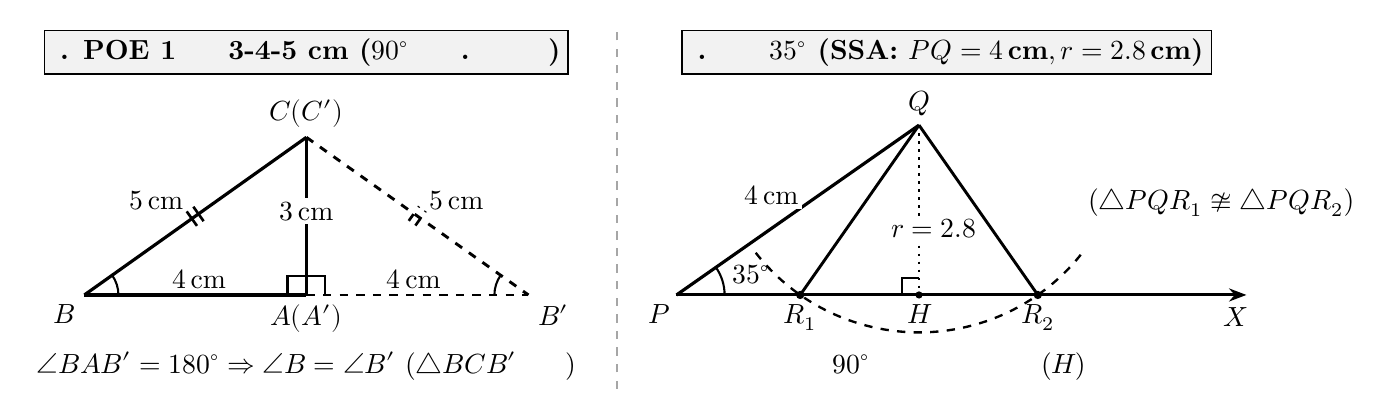
\begin{tikzpicture}[x=0.94cm, y=0.94cm, every node/.style={font=\linespread{1.0}\fontsize{10pt}{13.8pt}\selectfont, text=black}]
  % Panel Divider & Headers
  \draw[line width=0.6pt, dashed, gray!70] (8.35, 0.05) -- (8.35, 4.92);
  \node[anchor=north, fill=headgray, draw=black, line width=0.5pt, inner sep=2.8pt] at (4.15, 4.90) {\textbf{ក. \en{POE 1}៖ បត់ \en{3-4-5 cm} ($90^\circ$ ឱ្យ អ.ជ តែ ១ គូ)}};
  \node[anchor=north, fill=headgray, draw=black, line width=0.5pt, inner sep=2.8pt] at (12.80, 4.90) {\textbf{ខ. ល្បួង $35^\circ$ (\en{SSA}: $PQ=4\unit{cm}, r=2.8\unit{cm}$)}};

  % Left Panel: 3-4-5 Back-to-back Reflection
  \coordinate (A) at (4.15, 1.32);
  \coordinate (C) at (4.15, 3.45);
  \coordinate (B) at (1.15, 1.32);
  \coordinate (Bp) at (7.15, 1.32);
  \draw[line width=1.15pt, tk2] (B) -- (C);
  \draw[line width=1.05pt, dashed, tk2] (C) -- (Bp);
  \draw[line width=1.15pt, tk1] (A) -- (C);
  \draw[line width=1.15pt] (B) -- (A);
  \draw[line width=1.05pt, dashed] (A) -- (Bp);
  \rightanglemark[0.24]{(A)}{(B)}{(C)}
  \rightanglemark[0.24]{(A)}{(C)}{(Bp)}
  % Angle arcs at B and B'
  \draw[ang1] (B) ++(0:0.46) arc (0:35.37:0.46);
  \draw[ang1] (Bp) ++(180:0.46) arc (180:144.63:0.46);
  % Labels
  \node[above] at (C) {\en{$C(C')$}};
  \node[below] at (A) {\en{$A(A')$}};
  \node[below left] at (1.15, 1.32) {\en{$B$}};
  \node[below right] at (7.15, 1.32) {\en{$B'$}};
  \node[fill=white, inner sep=1.2pt] at (4.15, 2.45) {\en{$3\unit{cm}$}};
  \node[above left, inner sep=1.5pt] at (2.55, 2.40) {\en{$5\unit{cm}$}};
  \node[above right, inner sep=1.5pt] at (5.75, 2.40) {\en{$5\unit{cm}$}};
  \node[above, inner sep=1.2pt] at (2.70, 1.35) {\en{$4\unit{cm}$}};
  \node[above, inner sep=1.2pt] at (5.60, 1.35) {\en{$4\unit{cm}$}};
  \node[anchor=south] at (4.15, 0.04) {\en{$\ang{BAB'}=180^\circ \Rightarrow \ang{B}=\ang{B'}$} ($\tri{BCB'}$ សមបាទ)};

  % Right Panel: 35 deg SSA trap vs 90 deg
  \coordinate (P) at (9.15, 1.32);
  \coordinate (X) at (16.85, 1.32);
  \coordinate (Q) at (12.4266, 3.6143);
  \coordinate (H) at (12.4266, 1.32);
  \coordinate (R1) at (10.8215, 1.32);
  \coordinate (R2) at (14.0317, 1.32);
  \draw[line width=1.1pt, -{Stealth[length=2.2mm]}] (P) -- (X);
  \draw[line width=1.15pt] (P) -- (Q);
  \draw[line width=1.05pt] (Q) -- (R1);
  \draw[line width=1.05pt] (Q) -- (R2);
  \draw[line width=0.90pt, dotted] (Q) -- (H);
  \rightanglemark[0.22]{(H)}{(R1)}{(Q)}
  % Circle arc r = 2.80 around Q
  \draw[line width=0.85pt, dashed] ($(Q)+(-142:2.80)$) arc (-142:-38:2.80);
  \fill (R1) circle (1.5pt);
  \fill (R2) circle (1.5pt);
  \fill (H) circle (1.3pt);
  \draw[ang1] (P) ++(0:0.65) arc (0:35:0.65);
  \node[below left] at (P) {\en{$P$}};
  \node[inner sep=1pt] at ($(P)+(15:1.05)$) {\en{$35^\circ$}};
  \node[above] at (Q) {\en{$Q$}};
  \node[below] at (R1) {\en{$R_1$}};
  \node[below] at (H) {\en{$H$}};
  \node[below] at (R2) {\en{$R_2$}};
  \node[below] at (16.70, 1.28) {\en{$X$}};
  \node[fill=white, inner sep=1.2pt, above left] at (10.85, 2.48) {\en{$4\unit{cm}$}};
  \node[fill=white, inner sep=1.2pt, below left=1pt] at (13.28, 2.42) {\en{$r=2.8$}};
  \node[anchor=west, align=left] at (14.58, 2.68) {កាត់ ២ ត្រីកោណ\\($\tri{PQR_1} \ncg \tri{PQR_2}$)};
  \node[anchor=south] at (12.80, 0.04) {នៅ $90^\circ$ រង្វង់\textbf{ប៉ះតែ ១ ចំណុច} ($H$)};
\end{tikzpicture}\par
\vspace{12pt}
{\fontsize{10.5pt}{14pt}\selectfont\textbf{រូបទី ១៖} ការផ្ទៀង \en{POE 1} រវាងករណី \en{HL (3-4-5 cm)} តែមួយគត់ និងល្បួង $35^\circ$ (\en{SSA}) ដែលបាន ២ ត្រីកោណ \en{(Yigit Koyunkaya, 2018; Muzaini et al., 2023)}។}
\end{tcolorbox}

% --- រូបទី ២ ---
\begin{tcolorbox}[enhanced, sharp corners, colback=white, colframe=black, boxrule=0.8pt, top=5pt, bottom=4pt, left=4pt, right=4pt, before skip=4pt, after skip=6pt]
\centering
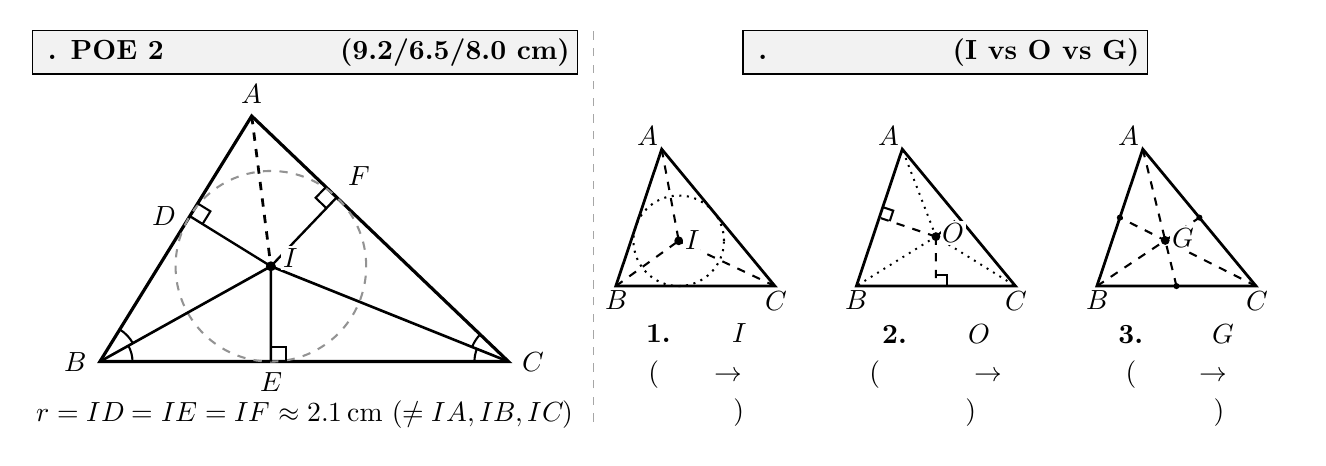
\begin{tikzpicture}[x=0.94cm, y=0.94cm, every node/.style={font=\linespread{1.0}\fontsize{10pt}{13.8pt}\selectfont, text=black}]
  \draw[line width=0.6pt, dashed, gray!70] (7.75, 0.05) -- (7.75, 5.36);
  \node[anchor=north, fill=headgray, draw=black, line width=0.5pt, inner sep=2.8pt] at (3.85, 5.34) {\textbf{ក. \en{POE 2}៖ បត់ត្រីកោណមិនសម័ង្ស (\en{9.2/6.5/8.0 cm})}};
  \node[anchor=north, fill=headgray, draw=black, line width=0.5pt, inner sep=2.8pt] at (12.50, 5.34) {\textbf{ខ. ការញែកផ្ចិត ៣ ប្រភេទ \en{(I vs O vs G)}}};

  % Left Panel: Proportional Scalene ABC + Incenter I + Inscribed circle + dashed AI
  \coordinate (B2) at (1.08, 0.86);
  \coordinate (C2) at (6.60, 0.86);
  \coordinate (A2) at (3.1308, 4.1773);
  \coordinate (I2) at (3.3900, 2.1477);
  \coordinate (D2) at ($(B2)!(I2)!(A2)$);
  \coordinate (E2) at (3.3900, 0.86);
  \coordinate (F2) at ($(A2)!(I2)!(C2)$);
  \draw[line width=1.15pt] (B2) -- (C2) -- (A2) -- cycle;
  \draw[line width=0.75pt, dashed, gray!85] (I2) circle (1.2877);
  \draw[line width=0.95pt] (B2) -- (I2) -- (C2);
  \draw[line width=1.00pt, dashed] (A2) -- (I2); % Strictly dashed AI
  \draw[line width=0.85pt] (I2) -- (D2) (I2) -- (E2) (I2) -- (F2);
  \rightanglemark[0.19]{(D2)}{(A2)}{(I2)}
  \rightanglemark[0.19]{(E2)}{(C2)}{(I2)}
  \rightanglemark[0.19]{(F2)}{(A2)}{(I2)}
  % Angle arcs at B and C ONLY (NEVER at A, NO / on AD,BD,BE,AF)
  \draw[ang1] (B2) ++(0:0.44) arc (0:29.1:0.44);
  \draw[ang1] (B2) ++(29.1:0.51) arc (29.1:58.2:0.51);
  \draw[ang1] (C2) ++(180:0.46) arc (180:158.1:0.46);
  \draw[ang1] (C2) ++(158.1:0.53) arc (158.1:136.3:0.53);
  \fill (I2) circle (1.8pt);
  \node[above=1pt] at (A2) {\en{$A$}};
  \node[left=1.5pt] at (B2) {\en{$B$}};
  \node[right=1.5pt] at (C2) {\en{$C$}};
  \node[left=1.5pt] at (D2) {\en{$D$}};
  \node[below=0.5pt] at (E2) {\en{$E$}};
  \node[above right=1pt] at (F2) {\en{$F$}};
  \node[fill=white, inner sep=1pt, right] at (3.52, 2.26) {\en{$I$}};
  \node[anchor=south] at (3.85, -0.18) {\en{$r = ID=IE=IF \approx 2.1\unit{cm}$ ($\ne IA,IB,IC$)}};

  % Right Panel: 3 Centers (I, O, G) spaced cleanly with 3-line captions
  \begin{scope}[shift={(8.05, 1.88)}]
    \coordinate (b1) at (0,0); \coordinate (c1) at (2.15,0); \coordinate (a1) at (0.62, 1.85);
    \coordinate (i1) at (0.8502, 0.6118);
    \draw[line width=1.0pt] (b1) -- (c1) -- (a1) -- cycle;
    \draw[line width=0.75pt, dashed] (a1) -- (i1) (b1) -- (i1) (c1) -- (i1);
    \draw[line width=0.75pt, dotted] (i1) circle (0.6118);
    \fill (i1) circle (1.6pt);
    \node[above left, inner sep=1pt] at (a1) {\en{$A$}};
    \node[below, inner sep=1.5pt] at (b1) {\en{$B$}};
    \node[below, inner sep=1.5pt] at (c1) {\en{$C$}};
    \node[fill=white, inner sep=0.8pt, right] at (0.90, 0.62) {\en{$I$}};
    \node[align=center, anchor=north, text width=2.85cm] at (1.075, -0.38) {\textbf{\en{1.} ផ្ចិត $I$}\\(ពុះមុំ $\to$\\ស្មើជ្រុង ៣)};
  \end{scope}

  \begin{scope}[shift={(11.30, 1.88)}]
    \coordinate (b2) at (0,0); \coordinate (c2) at (2.15,0); \coordinate (a2) at (0.62, 1.85);
    \coordinate (o2) at (1.075, 0.6686);
    \coordinate (mab) at (0.31, 0.925); \coordinate (mbc) at (1.075, 0); \coordinate (mac) at (1.385, 0.925);
    \draw[line width=1.0pt] (b2) -- (c2) -- (a2) -- cycle;
    \draw[line width=0.75pt, dashed] (o2) -- (mbc) (o2) -- (mab) (o2) -- (mac);
    \rightanglemark[0.14]{(mbc)}{(c2)}{(o2)}
    \rightanglemark[0.14]{(mab)}{(a2)}{(o2)}
    \rightanglemark[0.14]{(mac)}{(c2)}{(o2)}
    \draw[line width=0.7pt, dotted] (o2) -- (a2) (o2) -- (b2) (o2) -- (c2);
    \fill (o2) circle (1.6pt);
    \node[above left, inner sep=1pt] at (a2) {\en{$A$}};
    \node[below, inner sep=1.5pt] at (b2) {\en{$B$}};
    \node[below, inner sep=1.5pt] at (c2) {\en{$C$}};
    \node[fill=white, inner sep=0.8pt, right] at (1.13, 0.72) {\en{$O$}};
    \node[align=center, anchor=north, text width=2.85cm] at (1.075, -0.38) {\textbf{\en{2.} ផ្ចិត $O$}\\(ពុះកែងជ្រុង $\to$\\ស្មើកំពូល)};
  \end{scope}

  \begin{scope}[shift={(14.55, 1.88)}]
    \coordinate (b3) at (0,0); \coordinate (c3) at (2.15,0); \coordinate (a3) at (0.62, 1.85);
    \coordinate (g3) at (0.9233, 0.6167);
    \coordinate (mab3) at (0.31, 0.925); \coordinate (mbc3) at (1.075, 0); \coordinate (mac3) at (1.385, 0.925);
    \draw[line width=1.0pt] (b3) -- (c3) -- (a3) -- cycle;
    \draw[line width=0.75pt, dashed] (a3) -- (mbc3) (b3) -- (mac3) (c3) -- (mab3);
    \fill (g3) circle (1.6pt);
    \fill (mab3) circle (1.1pt) (mbc3) circle (1.1pt) (mac3) circle (1.1pt);
    \node[above left, inner sep=1pt] at (a3) {\en{$A$}};
    \node[below, inner sep=1.5pt] at (b3) {\en{$B$}};
    \node[below, inner sep=1.5pt] at (c3) {\en{$C$}};
    \node[fill=white, inner sep=0.8pt, right] at (0.98, 0.65) {\en{$G$}};
    \node[align=center, anchor=north, text width=2.85cm] at (1.075, -0.38) {\textbf{\en{3.} ទម្ងន់ $G$}\\(មេដ្យាន $\to$\\ចំណុចកណ្ដាល)};
  \end{scope}
\end{tikzpicture}\par
\vspace{2pt}
{\fontsize{10.5pt}{14pt}\selectfont\textbf{រូបទី ២៖} ការបត់ \en{POE 2} រកផ្ចិត $I$ លើត្រីកោណមិនសម័ង្ស និងតារាងរូបញែកផ្ចិតទាំង ៣ ($I, O, G$) \en{(Boz-Yaman, 2024; Demiray et al., 2023)}។}
\end{tcolorbox}

% --- រូបទី ៣ ---
\begin{tcolorbox}[enhanced, sharp corners, colback=white, colframe=black, boxrule=0.8pt, top=5pt, bottom=4pt, left=4pt, right=4pt, before skip=4pt, after skip=6pt]
\centering
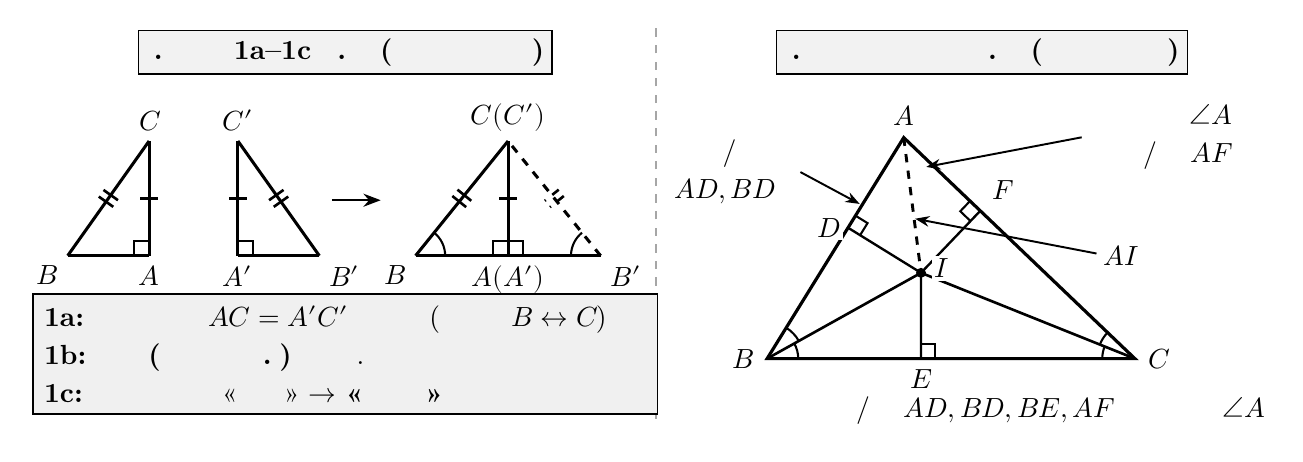
\begin{tikzpicture}[x=0.94cm, y=0.94cm, every node/.style={font=\linespread{1.0}\fontsize{10pt}{13.8pt}\selectfont, text=black}]
  \draw[line width=0.6pt, dashed, gray!70] (8.40, 0.05) -- (8.40, 5.32);
  \node[anchor=north, fill=headgray, draw=black, line width=0.5pt, inner sep=2.8pt] at (4.20, 5.30) {\textbf{ក. គំរូកែ \en{1a--1c} ទំ.១៥៤ (កុំសរសេររង្វង់តក្ក)}};
  \node[anchor=north, fill=headgray, draw=black, line width=0.5pt, inner sep=2.8pt] at (12.80, 5.30) {\textbf{ខ. គំរូកែរូបលំហាត់គំរូ ទំ.១៥៥ (ត្រីកោណមិនសម័ង្ស)}};

  % Left Panel: Fixed Book p.154
  \coordinate (A3) at (1.55, 2.25); \coordinate (C3) at (1.55, 3.80); \coordinate (B3) at (0.45, 2.25);
  \coordinate (Ap3) at (2.75, 2.25); \coordinate (Cp3) at (2.75, 3.80); \coordinate (Bp3) at (3.85, 2.25);
  \draw[line width=1.1pt, tk1] (A3) -- (C3);
  \draw[line width=1.1pt, tk2] (B3) -- (C3);
  \draw[line width=1.1pt] (B3) -- (A3);
  \draw[line width=1.1pt, tk1] (Ap3) -- (Cp3);
  \draw[line width=1.1pt, tk2] (Bp3) -- (Cp3);
  \draw[line width=1.1pt] (Bp3) -- (Ap3);
  \rightanglemark[0.19]{(A3)}{(B3)}{(C3)}
  \rightanglemark[0.19]{(Ap3)}{(Cp3)}{(Bp3)}
  \node[above] at (C3) {\en{$C$}}; \node[below] at (A3) {\en{$A$}}; \node[below left] at (B3) {\en{$B$}};
  \node[above] at (Cp3) {\en{$C'$}}; \node[below] at (Ap3) {\en{$A'$}}; \node[below right] at (Bp3) {\en{$B'$}};

  \draw[-{Stealth[length=2.2mm]}, line width=0.9pt] (4.02, 3.00) -- (4.68, 3.00);

  \coordinate (AJ) at (6.40, 2.25); \coordinate (CJ) at (6.40, 3.80);
  \coordinate (BJ) at (5.15, 2.25); \coordinate (BpJ) at (7.65, 2.25);
  \draw[line width=1.1pt, tk1] (AJ) -- (CJ);
  \draw[line width=1.1pt, tk2] (BJ) -- (CJ);
  \draw[line width=1.1pt, dashed, tk2] (BpJ) -- (CJ);
  \draw[line width=1.1pt] (BJ) -- (AJ) -- (BpJ);
  \rightanglemark[0.19]{(AJ)}{(BJ)}{(CJ)}
  \rightanglemark[0.19]{(AJ)}{(CJ)}{(BpJ)}
  \draw[ang1] (BJ) ++(0:0.40) arc (0:51.1:0.40);
  \draw[ang1] (BpJ) ++(180:0.40) arc (180:128.9:0.40);
  \node[above] at (CJ) {\en{$C(C')$}}; \node[below] at (AJ) {\en{$A(A')$}};
  \node[below left] at (BJ) {\en{$B$}}; \node[below right] at (BpJ) {\en{$B'$}};

  \node[draw=black, fill=panelgray, line width=0.7pt, align=left, anchor=south, inner sep=4pt, text width=7.65cm] at (4.20, 0.10) {%
    \textbf{\en{1a}:} រក្សាជ្រុងកែង \en{$AC = A'C'$} ជាប់លាប់ (កុំប្ដូរ \en{$B \leftrightarrow C$})\\
    \textbf{\en{1b}:} សរសេរ \textbf{(តាមលក្ខខណ្ឌ អ.ម)} ជំនួស អ.ជ រង្វង់តក្ក\\
    \textbf{\en{1c}:} កែអក្ខរាវិរុទ្ធ «លកខណ្ឌ» $\to$ \textbf{«លក្ខខណ្ឌ»}};

  % Right Panel: Book p.155 Fixed Scalene Incenter Model (clean callouts)
  \coordinate (B3r) at (9.90, 0.86);
  \coordinate (C3r) at (14.868, 0.86);
  \coordinate (A3r) at (11.7457, 3.8456);
  \coordinate (I3r) at (11.9790, 2.0190);
  \coordinate (D3r) at ($(B3r)!(I3r)!(A3r)$);
  \coordinate (E3r) at (11.9790, 0.86);
  \coordinate (F3r) at ($(A3r)!(I3r)!(C3r)$);
  \draw[line width=1.15pt] (B3r) -- (C3r) -- (A3r) -- cycle;
  \draw[line width=0.95pt] (B3r) -- (I3r) -- (C3r);
  \draw[line width=1.05pt, dashed] (A3r) -- (I3r); % Strictly dashed AI
  \draw[line width=0.85pt] (I3r) -- (D3r) (I3r) -- (E3r) (I3r) -- (F3r);
  \rightanglemark[0.18]{(D3r)}{(A3r)}{(I3r)}
  \rightanglemark[0.18]{(E3r)}{(C3r)}{(I3r)}
  \rightanglemark[0.18]{(F3r)}{(A3r)}{(I3r)}
  % Bisector arcs ONLY at B and C (NO arcs at A, NO / on AD,BD,BE,AF)
  \draw[ang1] (B3r) ++(0:0.42) arc (0:29.1:0.42);
  \draw[ang1] (B3r) ++(29.1:0.49) arc (29.1:58.2:0.49);
  \draw[ang1] (C3r) ++(180:0.44) arc (180:158.1:0.44);
  \draw[ang1] (C3r) ++(158.1:0.51) arc (158.1:136.3:0.51);
  \fill (I3r) circle (1.8pt);
  \node[above=1pt] at (A3r) {\en{$A$}};
  \node[left=1.5pt] at (B3r) {\en{$B$}};
  \node[right=1.5pt] at (C3r) {\en{$C$}};
  \node[left=1.5pt, fill=white, inner sep=1pt] at (D3r) {\en{$D$}};
  \node[below=0.5pt] at (E3r) {\en{$E$}};
  \node[above right=1pt] at (F3r) {\en{$F$}};
  \node[fill=white, inner sep=1pt, right] at (12.12, 2.08) {\en{$I$}};
  % Clean non-overlapping Callout arrows
  \node[anchor=west, align=left] at (8.52, 3.38) {គ្មាន \en{/} លើ\\ \en{$AD, BD$}};
  \draw[-{Stealth[length=1.8mm]}, line width=0.7pt] (10.35, 3.38) -- (11.15, 2.95);
  \node[anchor=west, align=left] at (14.20, 3.85) {គ្មានធ្នូនៅ \en{$\ang{A}$}\\គ្មាន \en{/} លើ \en{$AF$}};
  \draw[-{Stealth[length=1.8mm]}, line width=0.7pt] (14.15, 3.85) -- (12.05, 3.45);
  \node[anchor=west, fill=white, inner sep=1pt] at (14.40, 2.25) {\en{$AI$} ដាច់ៗ};
  \draw[-{Stealth[length=1.8mm]}, line width=0.7pt] (14.35, 2.28) -- (11.90, 2.75);
  \node[anchor=south] at (12.80, -0.16) {\textbf{រូបមិនសម័ង្ស៖} គ្មាន \en{/} លើ \en{$AD, BD, BE, AF$} និងគ្មានធ្នូ $\ang{A}$};
\end{tikzpicture}\par
\vspace{2pt}
{\fontsize{10.5pt}{14pt}\selectfont\textbf{រូបទី ៣៖} ការជួសជុលកំហុស \en{1a--1c} ទំ.១៥៤ (ឆ្វេង) និងរូបគំរូកែលំហាត់គំរូ ទំ.១៥៥ (ស្ដាំ) \en{(Anwar et al., 2023; Tchonang Youkap et al., 2020)}។}
\end{tcolorbox}

% --- រូបទី ៤ ---
\begin{tcolorbox}[enhanced, sharp corners, colback=white, colframe=black, boxrule=0.8pt, top=5pt, bottom=4pt, left=4pt, right=4pt, before skip=4pt, after skip=6pt]
\centering
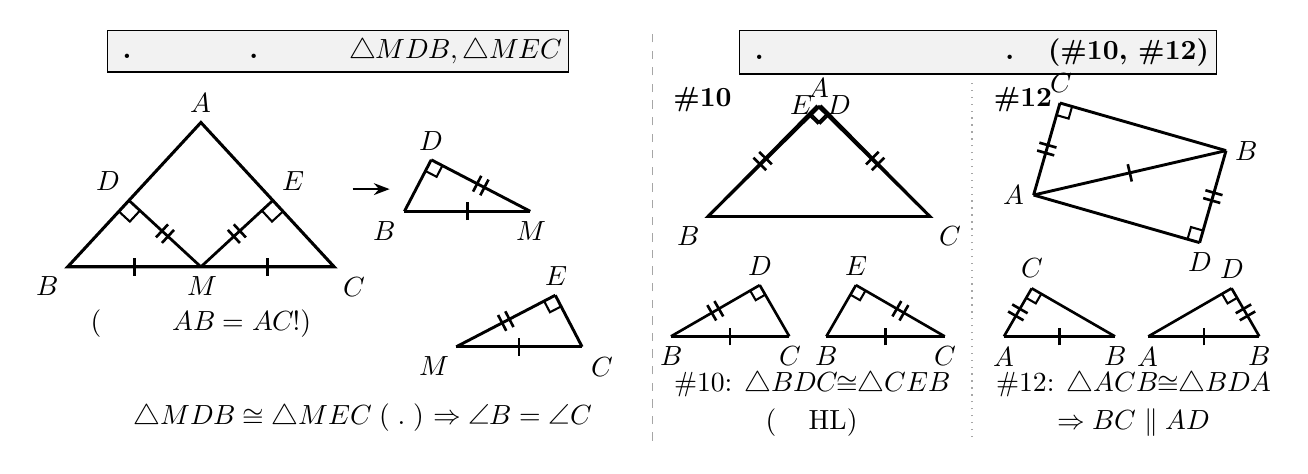
\begin{tikzpicture}[x=0.94cm, y=0.94cm, every node/.style={font=\linespread{1.0}\fontsize{10pt}{13.8pt}\selectfont, text=black}]
  \draw[line width=0.6pt, dashed, gray!70] (8.40, 0.05) -- (8.40, 5.62);
  \draw[line width=0.5pt, dotted, gray!70] (12.72, 0.10) -- (12.72, 4.95);
  \node[anchor=north, fill=headgray, draw=black, line width=0.5pt, inner sep=2.8pt] at (4.15, 5.60) {\textbf{ក. ប្រតិបត្តិ ទំ.១៥៦៖ បំបែក $\tri{MDB}, \tri{MEC}$}};
  \node[anchor=north, fill=headgray, draw=black, line width=0.5pt, inner sep=2.8pt] at (12.80, 5.60) {\textbf{ខ. បំបែកត្រួតគ្នាកិច្ចការផ្ទះ ទំ.១៦៥ (\en{\#10, \#12})}};

  % Left Panel: Pratibat p.156 (Main + Exploded)
  \coordinate (B4) at (0.50, 2.40); \coordinate (C4) at (4.10, 2.40); \coordinate (A4) at (2.30, 4.35);
  \coordinate (M4) at (2.30, 2.40);
  \coordinate (D4) at ($(A4)!(M4)!(B4)$); \coordinate (E4) at ($(A4)!(M4)!(C4)$);
  \draw[line width=1.1pt] (B4) -- (C4) -- (A4) -- cycle;
  \draw[line width=1.0pt, tk1] (B4) -- (M4);
  \draw[line width=1.0pt, tk1] (M4) -- (C4);
  \draw[line width=1.0pt, tk2] (M4) -- (D4);
  \draw[line width=1.0pt, tk2] (M4) -- (E4);
  \rightanglemark[0.19]{(D4)}{(B4)}{(M4)}
  \rightanglemark[0.19]{(E4)}{(C4)}{(M4)}
  \node[above] at (A4) {\en{$A$}}; \node[below left] at (B4) {\en{$B$}}; \node[below right] at (C4) {\en{$C$}};
  \node[below] at (M4) {\en{$M$}}; \node[above left] at (D4) {\en{$D$}}; \node[above right] at (E4) {\en{$E$}};
  \node[anchor=north] at (2.30, 1.95) {(ហាមសន្មត \en{$AB=AC$}!)};

  \draw[-{Stealth[length=2mm]}, line width=0.9pt] (4.35, 3.45) -- (4.85, 3.45);
  \coordinate (BM1) at (5.05, 3.15); \coordinate (MM1) at (6.75, 3.15); \coordinate (DM1) at (5.412, 3.846);
  \draw[line width=1.05pt, tk2] (MM1) -- (DM1);
  \draw[line width=1.05pt, tk1] (BM1) -- (MM1);
  \draw[line width=1.05pt] (DM1) -- (BM1);
  \rightanglemark[0.16]{(DM1)}{(BM1)}{(MM1)}
  \node[above] at (DM1) {\en{$D$}}; \node[below left] at (BM1) {\en{$B$}}; \node[below] at (MM1) {\en{$M$}};

  \coordinate (MM2) at (5.75, 1.32); \coordinate (CM3) at (7.45, 1.32); \coordinate (DM3) at (7.088, 2.016);
  \draw[line width=1.05pt, tk2] (MM2) -- (DM3);
  \draw[line width=1.05pt, tk1] (MM2) -- (CM3);
  \draw[line width=1.05pt] (DM3) -- (CM3);
  \rightanglemark[0.16]{(DM3)}{(MM2)}{(CM3)}
  \node[above] at (DM3) {\en{$E$}}; \node[below left] at (MM2) {\en{$M$}}; \node[below right] at (CM3) {\en{$C$}};
  \node[anchor=south, align=center] at (4.15, 0.04) {បំបែក $\tri{MDB}\cg\tri{MEC}$ (អ.ជ) $\Rightarrow \ang{B}=\ang{C}$};

  % Right Panel Top & Exploded: HW #10 and #12 cleanly separated
  % #10 at x=8.55..12.50
  \coordinate (B10) at (9.15, 3.08); \coordinate (C10) at (12.15, 3.08); \coordinate (A10) at (10.65, 4.56);
  \coordinate (D10) at ($(A10)!(B10)!(C10)$); \coordinate (E10) at ($(A10)!(C10)!(B10)$);
  \draw[line width=1.05pt] (B10) -- (C10) -- (A10) -- cycle;
  \draw[line width=1.0pt, tk2] (B10) -- (D10);
  \draw[line width=1.0pt, tk2] (C10) -- (E10);
  \rightanglemark[0.16]{(D10)}{(C10)}{(B10)}
  \rightanglemark[0.16]{(E10)}{(B10)}{(C10)}
  \node[above] at (A10) {\en{$A$}}; \node[below left] at (B10) {\en{$B$}}; \node[below right] at (C10) {\en{$C$}};
  \node[right] at (D10) {\en{$D$}}; \node[left] at (E10) {\en{$E$}};
  \node[anchor=west] at (8.55, 4.66) {\textbf{\en{\#10}}};

  \coordinate (b10a) at (8.65, 1.46); \coordinate (c10a) at (10.25, 1.46); \coordinate (d10a) at (9.85, 2.1528);
  \draw[line width=0.95pt, tk1] (b10a) -- (c10a);
  \draw[line width=0.95pt, tk2] (b10a) -- (d10a);
  \draw[line width=0.95pt] (d10a) -- (c10a);
  \rightanglemark[0.14]{(d10a)}{(b10a)}{(c10a)}
  \node[below] at (b10a) {\en{$B$}}; \node[below] at (c10a) {\en{$C$}}; \node[above] at (d10a) {\en{$D$}};

  \coordinate (b10b) at (10.75, 1.46); \coordinate (c10b) at (12.35, 1.46); \coordinate (e10b) at (11.15, 2.1528);
  \draw[line width=0.95pt, tk1] (b10b) -- (c10b);
  \draw[line width=0.95pt, tk2] (c10b) -- (e10b);
  \draw[line width=0.95pt] (b10b) -- (e10b);
  \rightanglemark[0.14]{(e10b)}{(b10b)}{(c10b)}
  \node[below] at (b10b) {\en{$B$}}; \node[below] at (c10b) {\en{$C$}}; \node[above] at (e10b) {\en{$E$}};
  \node[anchor=south, align=center] at (10.55, -0.02) {\en{\#10: \tri{BDC}\cg\tri{CEB}}\\(តាម \en{HL})};

  % #12 at x=12.88..17.00
  \coordinate (A12) at (13.55, 3.37); \coordinate (B12) at (16.15, 3.97);
  \coordinate (C12) at (13.9066, 4.6134); \coordinate (D12) at (15.7934, 2.7266);
  \draw[line width=1.05pt, tk1] (A12) -- (B12);
  \draw[line width=1.05pt, tk2] (A12) -- (C12);
  \draw[line width=1.05pt, tk2] (B12) -- (D12);
  \draw[line width=1.05pt] (C12) -- (B12) (A12) -- (D12);
  \rightanglemark[0.16]{(C12)}{(A12)}{(B12)}
  \rightanglemark[0.16]{(D12)}{(B12)}{(A12)}
  \node[left] at (A12) {\en{$A$}}; \node[right] at (B12) {\en{$B$}};
  \node[above] at (C12) {\en{$C$}}; \node[below] at (D12) {\en{$D$}};
  \node[anchor=west] at (12.88, 4.66) {\textbf{\en{\#12}}};

  \coordinate (a12a) at (13.15, 1.46); \coordinate (b12a) at (14.65, 1.46); \coordinate (c12a) at (13.525, 2.1095);
  \draw[line width=0.95pt, tk1] (a12a) -- (b12a);
  \draw[line width=0.95pt, tk2] (a12a) -- (c12a);
  \draw[line width=0.95pt] (c12a) -- (b12a);
  \rightanglemark[0.14]{(c12a)}{(a12a)}{(b12a)}
  \node[below] at (a12a) {\en{$A$}}; \node[below] at (b12a) {\en{$B$}}; \node[above] at (c12a) {\en{$C$}};

  \coordinate (a12b) at (15.10, 1.46); \coordinate (b12b) at (16.60, 1.46); \coordinate (d12b) at (16.225, 2.1095);
  \draw[line width=0.95pt, tk1] (a12b) -- (b12b);
  \draw[line width=0.95pt, tk2] (b12b) -- (d12b);
  \draw[line width=0.95pt] (a12b) -- (d12b);
  \rightanglemark[0.14]{(d12b)}{(b12b)}{(a12b)}
  \node[below] at (a12b) {\en{$A$}}; \node[below] at (b12b) {\en{$B$}}; \node[above] at (d12b) {\en{$D$}};
  \node[anchor=south, align=center] at (14.90, -0.02) {\en{\#12: \tri{ACB}\cg\tri{BDA}}\\$\Rightarrow BC\parallel AD$};
\end{tikzpicture}\par
\vspace{2pt}
{\fontsize{10.5pt}{14pt}\selectfont\textbf{រូបទី ៤៖} ការគូរបំបែកត្រីកោណកែងត្រួតគ្នាក្នុងប្រតិបត្តិ ទំ.១៥៦ និងកិច្ចការផ្ទះ ទំ.១៦៥ (\en{\#10, \#12}) \en{(Biber, 2020)}។}
\end{tcolorbox}

% ============================================================================
% ផ្នែកទី ៦៖ មគ្គុទ្ទេសក៍រៀបចំ និងប្រើប្រាស់សម្ភារៈបោះពុម្ព (Pages 1--6) & ចម្លើយពេញលេញ
% ============================================================================
\secbanner{ផ្នែកទី ៦៖ មគ្គុទ្ទេសក៍រៀបចំ និងប្រើប្រាស់សម្ភារៈបោះពុម្ព \enbf{(Pages 1--6)}}{Section 6: Printing Calibration (Actual Size 100\%), Cut-Out Preparation \& Complete Answer Keys}

\subsec{៦\enbf{.}១ ស្តង់ដារបោះពុម្ព \enbf{Actual Size 100\%} និងលំដាប់ចែកសន្លឹកកិច្ចការ}

\begin{enumerate}[leftmargin=0.65cm, itemsep=2.5pt]
  \item \textbf{ការកំណត់បោះពុម្ព \en{1:1} ដាច់ខាត (ទំព័រ ១)}៖ បោះពុម្ពឯកសារ \en{Printable\_Materials\_HL.pdf} ដោយជ្រើសរើស \textbf{\en{Actual Size / Scale 100\%}} (\emph{ហាមប្រើ} \en{Fit to Page / Shrink to Fit}) ហើយយកបន្ទាត់វាស់ផ្ទៀងបារពិនិត្យ \textbf{\en{5.0 cm}} លើទំព័រ ១។ ទំព័រ ២, ៣ ជាទម្រង់ \en{2-up} (២ សន្លឹកក្នុង ១ ទំព័រ \en{A4}), ទំព័រ ៥ និង ៦ ជាទម្រង់ \en{4-up} (កាត \en{A--D} និងប័ណ្ណផ្ទះ)។
  \item \textbf{ក្រដាសផ្ទាំងគោល (ទំព័រ ៤)}៖ គួរបោះពុម្ពលើក្រដាសរឹង \en{180 gsm} ឬ \en{A4} ធម្មតាសម្រាប់បិទលើក្ដារខៀនកណ្ដាលពេញមេរៀន។
  \item \textbf{ឧបករណ៍តុក្រុម}៖ កន្ត្រៃ ១, បន្ទាត់ \en{mm} ១, រ៉ាព័រទ័រ និងដែកឈាន ១ ក្នុងមួយក្រុម (\en{3} នាក់)។ ចែកទំព័រ ១ ផ្កាប់ចុះក្រោមមុនម៉ោង (\en{00'}), ចែកទំព័រ ២ នៅនាទី ២៨', ចែកទំព័រ ៣ នៅនាទី ៣៨', លើកកាតទំព័រ ៥ នៅនាទី ៤៥', និងចែកទំព័រ ៦ នៅនាទី ៤៨'។
\end{enumerate}

\Needspace{2.0cm}
\subsec{៦\enbf{.}២ ចម្លើយគំរូពេញលេញសម្រាប់គ្រប់សន្លឹកកិច្ចការ និងលំហាត់ \enbf{(Pages 1--6 \& HW)}}

\begingroup
\linespread{1.05}\fontsize{10.5pt}{15.5pt}\selectfont
\begin{longtable}{|L{2.90cm}|L{13.95cm}|}
\hline
\rowcolor{headgray}
\multicolumn{1}{|C{2.90cm}|}{\tblhead{សន្លឹក \enbf{/} លំហាត់}} &
\multicolumn{1}{C{13.95cm}|}{\tblhead{ចម្លើយគំរូផ្លូវការ និងពិន្ទុត្រួតពិនិត្យ \enbf{(Master Key)}}} \\
\hline
\endfirsthead
\hline
\rowcolor{headgray}
\multicolumn{1}{|C{2.90cm}|}{\tblhead{សន្លឹក \enbf{/} លំហាត់}} &
\multicolumn{1}{C{13.95cm}|}{\tblhead{ចម្លើយគំរូផ្លូវការ និងពិន្ទុត្រួតពិនិត្យ \enbf{(Master Key)}}} \\
\hline
\endhead
\hline
\endfoot
\hline
\endlastfoot
\textbf{ទំព័រ ១ (\en{POE 1--2})} &
\textbf{ស.១}៖ កាត់ \en{3-4-5 cm} បង្វិល \en{195°} ផ្គុំ $A'C'=AC=3\unit{cm} \Rightarrow \ang{BAB'}=180^\circ \Rightarrow \tri{BCB'}$ សមបាទ ($\ang{B}=\ang{B'}$) $\Rightarrow \tri{ABC}\cg\tri{A'B'C'}$ តែមួយគត់ (តាម \textbf{អ.ម})។ នៅ $35^\circ$ ($PQ=4\unit{cm}, r=2.8\unit{cm}$), ធ្នូកាត់ $PX$ ត្រង់ \textbf{២ ចំណុច $R_1, R_2$} ($\tri{PQR_1}\ncg\tri{PQR_2}$)។ \newline
\textbf{ស.២}៖ $\tri{ABC}$ មិនសម័ង្ស (\en{9.2/6.5/8.0 cm})៖ បន្ទាត់បត់ $AI$ ពុះ $\ang{A}$ ត្រង់ចំផ្នត់! វាស់ $r = ID=IE=IF \approx 2.1\unit{cm}$ (កាំរង្វង់ចារឹកក្នុង), ចំណែក $IA \approx 3.4\unit{cm}, IB \approx 4.4\unit{cm}, IC \approx 5.8\unit{cm}$ (មិនស្មើគ្នា)។ \\
\hline
\textbf{ទំព័រ ២ (\en{E4})} \newline លំហាត់គំរូ ទំ.១៥៥ &
\textbf{ដំណាក់កាល ១}៖ $\tri{BEI}\cg\tri{BDI}$ (អ.ម៖ $90^\circ$, $BI$ រួម, $\ang{EBI}=\ang{DBI}$) $\Rightarrow ID=IE$; $\tri{CEI}\cg\tri{CFI}$ (អ.ម) $\Rightarrow IE=IF \Rightarrow ID=IF$។ \newline
\textbf{ដំណាក់កាល ២}៖ ក្នុង $\tri{IDA}, \tri{IFA}$៖ $\ang{IDA}=\ang{IFA}=90^\circ$ (\cnum{1}), $AI$ រួមឈម $90^\circ$ (\cnum{2}), $ID=IF$ ពីដំណាក់កាល ១ (\cnum{3}) $\Rightarrow \tri{IDA}\cg\tri{IFA}$ (\cnum{4} អ.ជ) $\Rightarrow \ang{IAD}=\ang{IAF}$ (\cnum{5}) $\Rightarrow AI$ ពុះ $\ang{BAC}$។ \textbf{\en{EIA 30s}}៖ $ID=IE=IF \ne IA,IB,IC$; គ្មាន \en{/} លើ $AD, BD, BE, AF$។ \\
\hline
\textbf{ទំព័រ ៣ (\en{E5})} \newline ប្រតិបត្តិ ទំ.១៥៦ &
\textbf{បម្រាប់}៖ $M$ ចំណុចកណ្ដាល $BC$, $MD\perp AB$, $ME\perp AC$, $MD=ME$។ ក្នុង $\tri{MDB}, \tri{MEC}$៖ $\ang{MDB}=\ang{MEC}=90^\circ$ (\cnum{1} អង្កត់កែង), អ៊ីប៉ូតេនុស $MB=MC$ (\cnum{2} ចំណុចកណ្ដាល), ជ្រុងកែង $MD=ME$ (\cnum{3} បម្រាប់) $\Rightarrow \tri{MDB}\cg\tri{MEC}$ (\cnum{4} អ.ជ) $\Rightarrow \ang{B}=\ang{C}$ (\cnum{5} មុំត្រូវគ្នា)។ \textbf{បិទ \en{E1}}៖ អាងទឹកនៅត្រង់ $I$ ព្រោះ $ID=IE=IF$។ \\
\hline
\textbf{ទំព័រ ៥ (កាត \en{A--D})} &
\textbf{កាត \en{A} (\ding{51} អ.ជ)}៖ បង្វិល $\sim 140^\circ$, មាន $\ang{A}=\ang{D}=90^\circ$, អ៊ីប៉ូតេនុស $BC=EF$, ជ្រុងកែង $AC=DF$។ \newline
\textbf{កាត \en{B} ($\times$ ល្បួង \en{SSA})}៖ មុំ $60^\circ \ne 90^\circ$ (ជ្រុង $4\unit{cm}$ ជាប់ $\ang{P}=\ang{P'}=60^\circ$ ដូចគ្នា, តែជ្រុង $5\unit{cm}$ ប្ដូរពីជាប់ $PR=5\unit{cm}$ [\en{SAS}] ទៅឈម $Q'R'=5\unit{cm}$ [\en{SSA}] $\Rightarrow P'R'\approx 5.61\unit{cm}$) មិនអាចប្រើ \en{HL} ទេ។ \newline
\textbf{កាត \en{C} ($\times$ ច្រឡំផ្ចិត)}៖ ផ្ចិត $I$ ស្មើចម្ងាយពីជ្រុង ($ID=IE=IF$) មិនមែន $IA=IB=IC$ (នោះជាផ្ចិត $O$)។ \newline
\textbf{កាត \en{D} ($\times$ អ៊ីប៉ូ vs កែង)}៖ $\tri{KLM}$ កែងត្រង់ $K$ ដូច្នេះ $LM=5\unit{cm}$ ជា\emph{អ៊ីប៉ូតេនុស}, តែ $\tri{K'L'M'}$ កែងត្រង់ $K'$ ដូច្នេះ $K'M'=5\unit{cm}$ ជា\emph{ជ្រុងកែង} ($\Rightarrow L'M'\approx 5.83\unit{cm} \ne 5$)។ \\
\hline
\textbf{ទំព័រ ៦ (ផ្ទះ)} \newline ទំ.១៦៥ \en{\#10, \#12} &
\textbf{រំលឹក \en{\#6, \#7}}៖ \en{\#6} = \textbf{ម.ជ.ម (\en{ASA})}; \en{\#7} ក. = \textbf{ជ.ម.ជ (\en{SAS})}, ខ. = \textbf{អ.ម (\en{HA})}។ \newline
\textbf{លំហាត់ \en{\#10}} (បន្ថែម \en{[AC} និង \en{AB]} ក្រោយ «កាត់ជ្រុងឈម»)៖ បំបែក $\tri{BDC}, \tri{CEB}$៖ $\ang{BDC}=\ang{CEB}=90^\circ$ (\cnum{1}), អ៊ីប៉ូតេនុសរួម $BC=CB$ (\cnum{2}), ជ្រុងកែង $BD=CE$ (\cnum{3}) $\Rightarrow \tri{BDC}\cg\tri{CEB}$ (\cnum{4} អ.ជ) $\Rightarrow \ang{DCB}=\ang{EBC}$ (\cnum{5} មុំឈមជ្រុង $BD=CE$) $\Rightarrow \ang{ABC}=\ang{ACB}$។ \newline
\textbf{លំហាត់ \en{\#12}}៖ បំបែក $\tri{ACB}, \tri{BDA}$៖ $\ang{C}=\ang{D}=90^\circ$ (\cnum{1}), អ៊ីប៉ូតេនុសរួម $AB=BA$ (\cnum{2}), ជ្រុងកែង $AC=BD$ (\cnum{3}) $\Rightarrow \tri{ACB}\cg\tri{BDA}$ (\cnum{4} អ.ជ) $\Rightarrow BC=AD$ និង $\ang{CBA}=\ang{DAB}$ (\cnum{5}) $\Rightarrow$ មុំឆ្លាស់ក្នុងស្មើគ្នា $\Rightarrow BC\parallel AD$។ \\
\hline
\end{longtable}
\endgroup

% ============================================================================
% ផ្នែកទី ៧៖ ឯកសារយោង (References --- APA 7th Edition) & ហត្ថលេខា
% ============================================================================
\refbanner{ឯកសារយោង}

{\TimesEn\linespread{1.0}\selectfont\fontsize{10.8pt}{16.2pt}\selectfont
\setlength{\parskip}{1.8pt}
\everypar={\hangindent=0.85cm \hangafter=1}

Anwar, L., Goedhart, M. J., \& Mali, A. (2023). Learning trajectory of geometry proof construction: Studying the emerging understanding of the structure of Euclidean proof. \textit{EURASIA Journal of Mathematics, Science and Technology Education}, \textit{19}(5), em2266. \url{https://doi.org/10.29333/ejmste/13160}

Anwar, L., Mali, A., \& Goedhart, M. J. (2021). The effect of proof format on reading comprehension of geometry proof: The case of Indonesian prospective mathematics teachers. \textit{EURASIA Journal of Mathematics, Science and Technology Education}, \textit{17}(4), em1952. \url{https://doi.org/10.29333/ejmste/10782}

Biber, A. Ç. (2020). Students' difficulties in similar triangle questions. \textit{Cypriot Journal of Educational Sciences}, \textit{15}(5), 1146--1159. \url{https://doi.org/10.18844/cjes.v15i5.5161}

Boz-Yaman, B. (2024). Effects of using patty paper practices during geometric constructions on attitude, self-efficacy, and achievement in geometry. \textit{Electronic Journal for Research in Science \& Mathematics Education}, \textit{28}(3), 1--15. \url{https://files.eric.ed.gov/fulltext/EJ1459697.pdf}

Demiray, E., Işıksal-Bostan, M., \& Saygı, E. (2023). How argumentation relates to formal proof process in geometry. \textit{International Electronic Journal of Mathematics Education}, \textit{18}(3), em0741. \url{https://doi.org/10.29333/iejme/13214}

Manalo, L. O. (2025). Geometric proof competencies of Grade 8 students. \textit{Psychology and Education: A Multidisciplinary Journal}, \textit{43}(9), 1148--1174. \url{https://doi.org/10.70838/pemj.430906}

Masinading, Z. M. B., \& Gaylo, D. N. (2022). Differentiated scaffolding strategies in triangle congruence: Their effects on learners' academic performance and confidence in mathematics. \textit{International Journal of Education and Literacy Studies}, \textit{10}(2), 131--140. \url{https://doi.org/10.7575/aiac.ijels.v.10n.2p.131}

Miyazaki, M., Nagata, J., Chino, K., Sasa, H., Fujita, T., Komatsu, K., \& Shimizu, S. (2019). Curriculum development for explorative proving in lower secondary school geometry: Focusing on the levels of planning and constructing a proof. \textit{Frontiers in Education}, \textit{4}, 31. \url{https://doi.org/10.3389/feduc.2019.00031}

Muzaini, M., Rahayuningsih, S., Ikram, M., \& Nasiruddin, F. A.-Z. (2023). Mathematical creativity: Student geometrical figure apprehension in geometry problem-solving using new auxiliary elements. \textit{International Journal of Educational Methodology}, \textit{9}(1), 139--150. \url{https://doi.org/10.12973/ijem.9.1.139}

Šipuš, Ž. M., Bašić, M., Doorman, M., Špalj, E., \& Antoliš, S. (2022). MERIA -- Conflict lines: Experience with two innovative teaching materials. \textit{Center for Educational Policy Studies Journal}, \textit{12}(1), 103--124. \url{https://doi.org/10.26529/cepsj.987}

Tchonang Youkap, P., Njomgang Ngansop, J., Tieudjo, D., \& Pedemonte, B. (2020). The introduction of proof at the secondary school in Cameroun: A first approach trough the study of quadrilaterals and triangles in the textbook. \textit{International Electronic Journal of Mathematics Education}, \textit{15}(3), em0599. \url{https://doi.org/10.29333/iejme/8404}

Winer, M. L., \& Battista, M. T. (2022). Investigating students' proof reasoning: Analyzing students' oral proof explanations and their written proofs in high school geometry. \textit{International Electronic Journal of Mathematics Education}, \textit{17}(2), em0677. \url{https://doi.org/10.29333/iejme/11713}

Yeo, L.-M., \& Tzeng, Y.-T. (2019). Tracing effect in the worked examples-based learning: An exploration of individual differences in working memory capacity. \textit{EURASIA Journal of Mathematics, Science and Technology Education}, \textit{15}(10), em1760. \url{https://doi.org/10.29333/ejmste/105482}

Yigit Koyunkaya, M. (2018). An examination of a pre-service mathematics teacher's mental constructions of relationships in a right triangle. \textit{International Journal of Education in Mathematics, Science and Technology}, \textit{6}(1), 58--78. \url{https://doi.org/10.18404/ijemst.328344}
\par}

\vspace{14pt}
\Needspace{2.0cm}
\hfill
\begin{minipage}{9.8cm}
  {\centering
    ថ្ងៃចន្ទ ៦រោច ខែកត្តិក ឆ្នាំមមី អដ្ឋស័ក ពុទ្ធសករាជ ២៥៧០\\[2pt]
    ត្រូវនឹងថ្ងៃទី៣០ ខែវិច្ឆិកា ឆ្នាំ២០២៦\\[3pt]
    {\muol គ្រូបង្រៀន}\par}
  \vspace{32pt}
  \hfill{\muol ហុក ប៊ុនថែន}\hspace*{1.4cm}
\end{minipage}

\end{document}
